% A LaTeX template for EXECUTIVE SUMMARY of the MSc Thesis submissions to 
% Politecnico di Milano (PoliMi) - School of Industrial and Information Engineering
%
% S. Bonetti, A. Gruttadauria, G. Mescolini, A. Zingaro
% e-mail: template-tesi-ingind@polimi.it
%
% Last Revision: October 2021
%
% Copyright 2021 Politecnico di Milano, Italy. NC-BY

\documentclass[11pt,a4paper,twocolumn]{article}

%------------------------------------------------------------------------------
%	REQUIRED PACKAGES AND  CONFIGURATIONS
%------------------------------------------------------------------------------
% PACKAGES FOR TITLES
\usepackage{titlesec}
\usepackage{color}

% PACKAGES FOR LANGUAGE AND FONT
% \usepackage[utf8]{inputenc}
% \usepackage[english]{babel}
% \usepackage[T1]{fontenc} % Font encoding
\usepackage[no-math]{fontspec}
\setmainfont{Latin Modern Roman}

% PACKAGES FOR IMAGES
\usepackage{graphicx}
\graphicspath{{Images/}} % Path for images' folder
\usepackage{eso-pic} % For the background picture on the title page
\usepackage{subfig} % Numbered and caption subfigures using \subfloat
\usepackage{caption} % Coloured captions
% \usepackage{transparent}
\usepackage{tikz}

% STANDARD MATH PACKAGES
\usepackage{amsfonts}
\usepackage{amssymb}
\usepackage{amsmath}
\usepackage{amsthm}
\usepackage{bm}
\usepackage[overload]{empheq}  % For braced-style systems of equations

% PACKAGES FOR TABLES
\usepackage{tabularx}
\usepackage{longtable} % tables that can span several pages
\usepackage{colortbl}

% PACKAGES FOR ALGORITHMS (PSEUDO-CODE)
\usepackage{algorithm}
\usepackage{algorithmic}

% PACKAGES FOR REFERENCES & BIBLIOGRAPHY
\usepackage[colorlinks=true,linkcolor=black,anchorcolor=black,citecolor=black,filecolor=black,menucolor=black,runcolor=black,urlcolor=black]{hyperref} % Adds clickable links at references
\usepackage{cleveref}
\usepackage[square, numbers, sort&compress]{natbib} % Square brackets, citing references with numbers, citations sorted by appearance in the text and compressed
\bibliographystyle{plain} % You may use a different style adapted to your field

% PACKAGES FOR THE APPENDIX
\usepackage{appendix}

% PACKAGES FOR ITEMIZE & ENUMERATES 
\usepackage{enumitem}

% OTHER PACKAGES
\usepackage{amsthm,thmtools,xcolor} % Coloured "Theorem"
\usepackage{comment} % Comment part of code
\usepackage{fancyhdr} % Fancy headers and footers
\usepackage{lipsum} % Insert dummy text
\usepackage{tcolorbox} % Create coloured boxes (e.g. the one for the key-words)
\usepackage{stfloats} % Correct position of the tables

\definecolor{bluepoli}{cmyk}{0.4,0.1,0,0.4}

%-------------------------------------------------------------------------
%	NEW COMMANDS DEFINED
%-------------------------------------------------------------------------
% EXAMPLES OF NEW COMMANDS -> here you see how to define new commands
\newcommand{\bea}{\begin{eqnarray}} % Shortcut for equation arrays
\newcommand{\eea}{\end{eqnarray}}
\newcommand{\e}[1]{\times 10^{#1}}  % Powers of 10 notation
\newcommand{\mathbbm}[1]{\text{\usefont{U}{bbm}{m}{n}#1}} % From mathbbm.sty
\newcommand{\pdev}[2]{\frac{\partial#1}{\partial#2}}
% NB: you can also override some existing commands with the keyword \renewcommand

%----------------------------------------------------------------------------
%	ADD YOUR PACKAGES (be careful of package interaction)
%----------------------------------------------------------------------------


%----------------------------------------------------------------------------
%	ADD YOUR DEFINITIONS AND COMMANDS (be careful of existing commands)
%----------------------------------------------------------------------------


% Do not change Configuration_files/config.tex file unless you really know what you are doing. 
% This file ends the configuration procedures (e.g. customizing commands, definition of new commands)
% Set the geometric layout of the document
\usepackage{geometry}
\geometry{
  top=3cm,
  left = 2.0cm,
  right = 2.0cm,
  bottom=2cm,
  headheight= 2cm,
  headsep= 0cm,
}
\raggedbottom 

% Create color bluePoli (-> manuale grafica coordinata:  https://www.polimi.it/fileadmin/user_upload/il_Politecnico/grafica-coordinata/2015_05_11_46xy_manuale_grafica_coordinata.pdf)
\definecolor{bluePoli}{cmyk}{0.4,0.1,0,0.4}

% Custom theorem environments
\declaretheoremstyle[
  headfont=\color{bluePoli}\normalfont\bfseries,
  bodyfont=\color{black}\normalfont\itshape,
]{colored}

\captionsetup[figure]{labelfont={color=bluePoli}} % Set colour of the captions
\captionsetup[table]{labelfont={color=bluePoli}} % Set colour of the captions
\captionsetup[algorithm]{labelfont={color=bluePoli}} % Set colour of the captions

\theoremstyle{colored}
\newtheorem{theorem}{Theorem}[section]
\newtheorem{proposition}{Proposition}[section]

% Enhances the features of the standard "table" and "tabular" environments.
\newcommand\T{\rule{0pt}{2.6ex}}
\newcommand\B{\rule[-1.2ex]{0pt}{0pt}}

% Algorithm description
\newcounter{algsubstate}
\renewcommand{\thealgsubstate}{\alph{algsubstate}}
\newenvironment{algsubstates}{
    \setcounter{algsubstate}{0}%
    \renewcommand{\STATE}{%
    \stepcounter{algsubstate}%
    \Statex {\small\thealgsubstate:}\space}
    }{}
    
% Custom theorem environment
\newcolumntype{L}[1]{>{\raggedright\let\newline\\\arraybackslash\hspace{0pt}}m{#1}}
\newcolumntype{C}[1]{>{\centering\let\newline\\\arraybackslash\hspace{0pt}}m{#1}}
\newcolumntype{R}[1]{>{\raggedleft\let\newline\\\arraybackslash\hspace{0pt}}m{#1}}

% Custom itemize environment
\setlist[itemize,1]{label=$\bullet$}
\setlist[itemize,2]{label=$\circ$}
\setlist[itemize,3]{label=$-$}
\setlist{nosep}

% Set separation of columns 
\setlength{\columnsep}{30pt}

% Create command for background pic
% \newcommand\BackgroundPic{% Adding background picture
% 	\put(210,350){
% 		\parbox[b][\paperheight]{\paperwidth}{%
% 			\vfill
% 			\centering
% 			\transparent{0.25}
% 			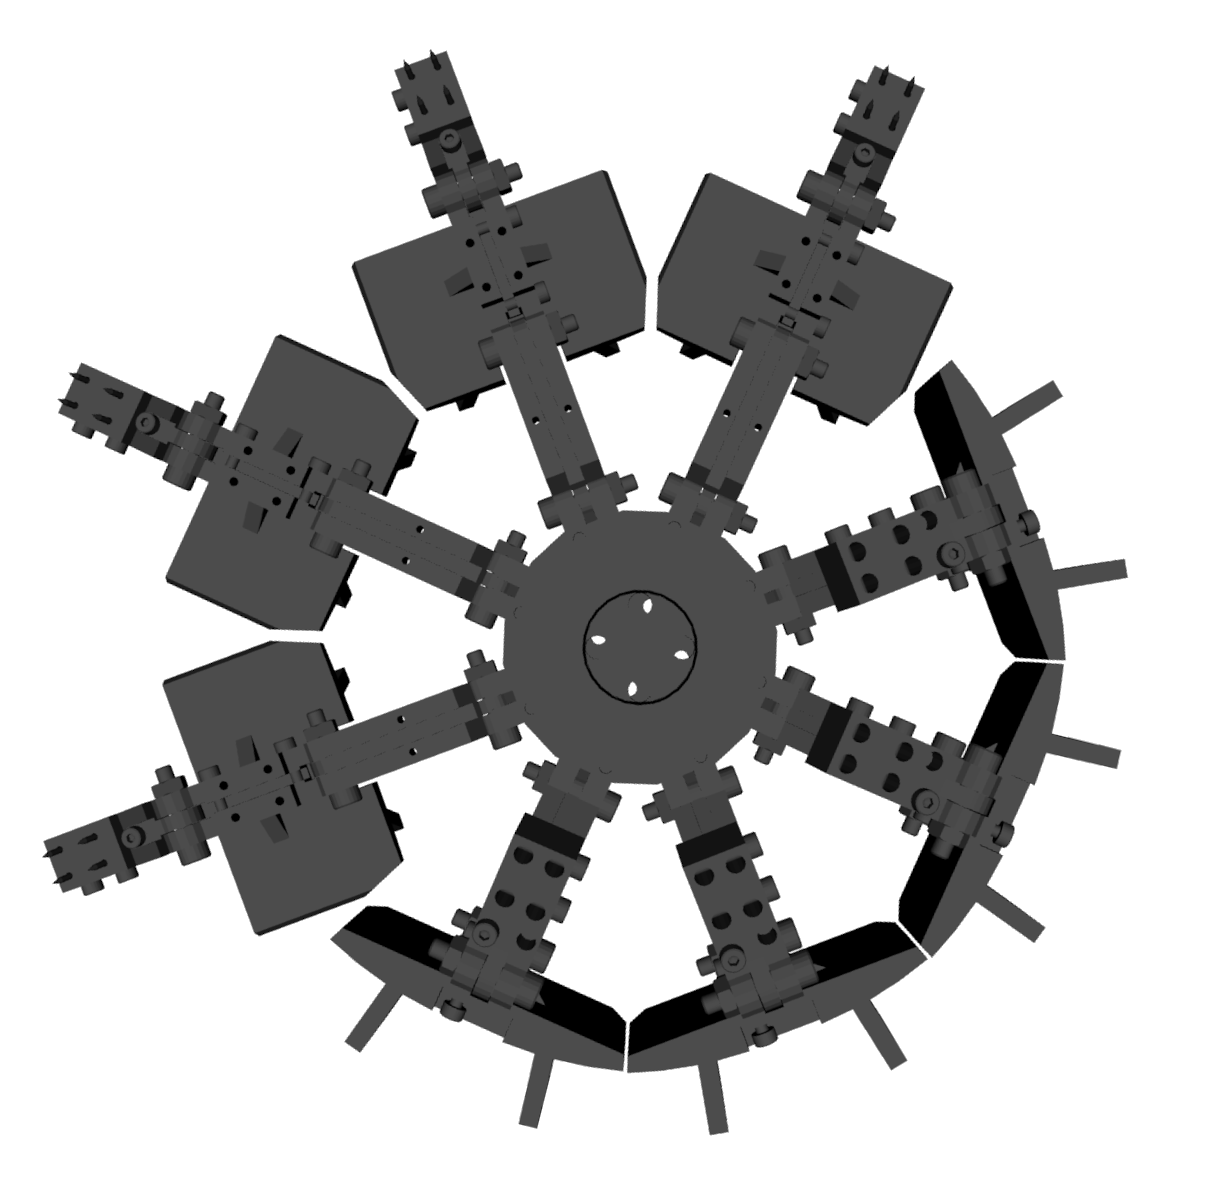
\includegraphics[width=0.55\paperwidth]{Images/GW_mixed_new.png}%
% 			\vfill
% }}}
\newcommand\BackgroundPic{%
	\put(225,355){%
		\parbox[b][\paperheight]{\paperwidth}{%
			\vfill
			\centering
			\tikz\node[opacity=0.25,inner sep=0pt]{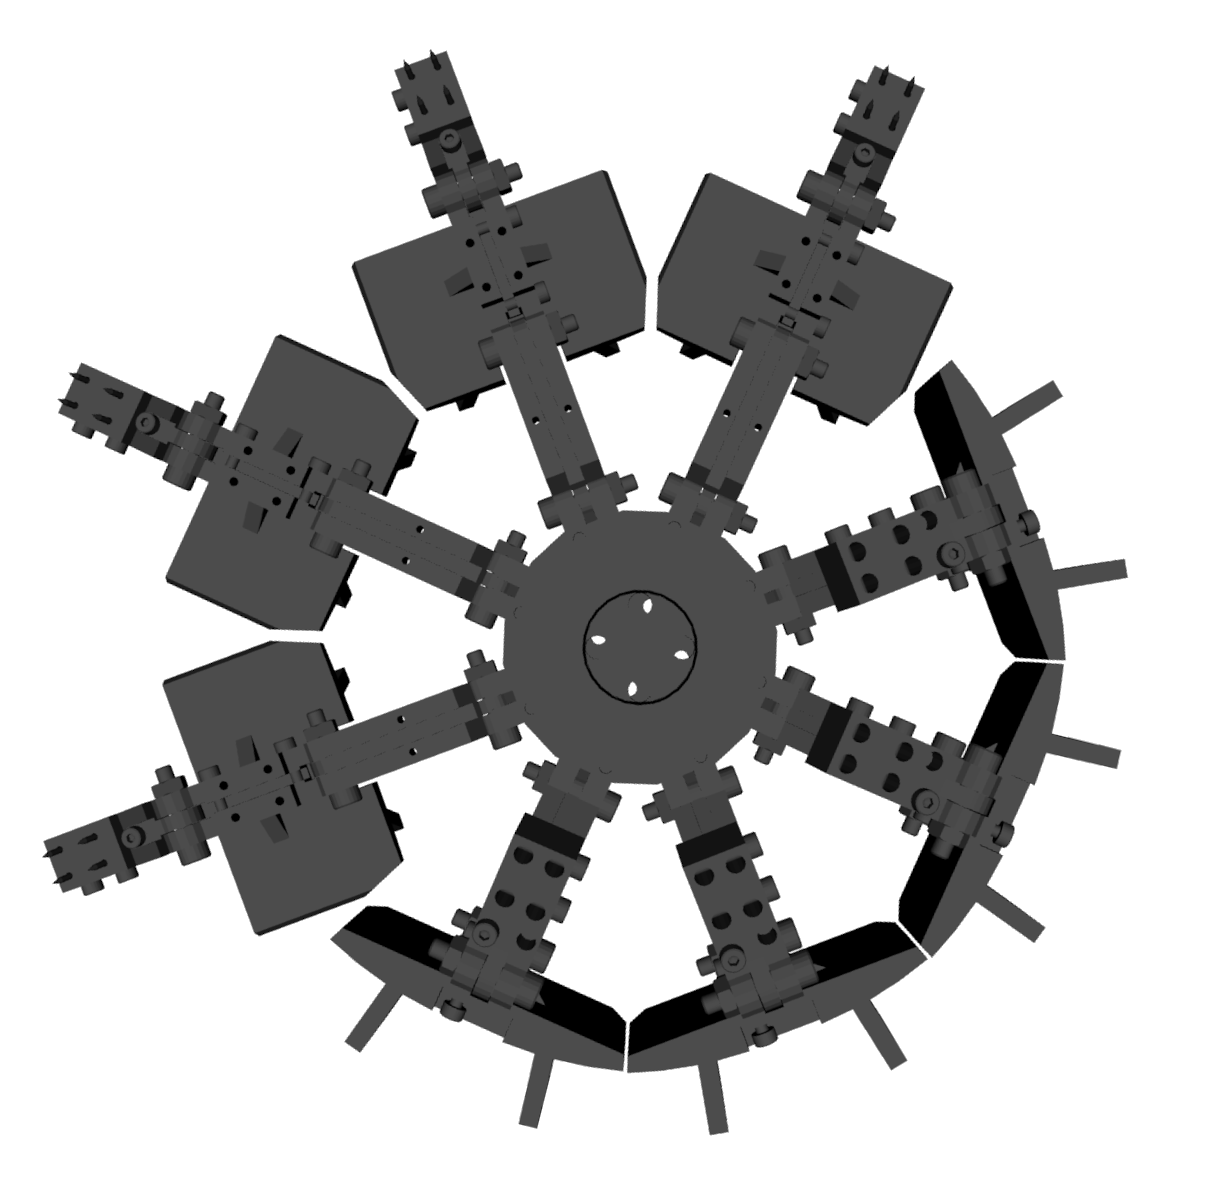
\includegraphics[width=0.55\paperwidth]{Images/GW_mixed_new.png}};
			\vfill
}}}

% Set indentation
\setlength\parindent{0pt}

% Custom title commands
\titleformat{\section}
{\color{bluePoli}\normalfont\Large\bfseries}
{\color{bluePoli}\thesection.}{1em}{}
\titlespacing*{\section}
{0pt}{2ex}{1ex}

\titleformat{\subsection}
{\color{bluePoli}\normalfont\large\bfseries}
{\color{bluePoli}\thesubsection.}{1em}{}
\titlespacing*{\subsection}
{0pt}{2ex}{1ex}

% Custom headers and footers
\pagestyle{fancy}
\fancyhf{}
      
\fancyfoot{}
\fancyfoot[C]{\thepage} % page
\renewcommand{\headrulewidth}{0mm} % headrule width
\renewcommand{\footrulewidth}{0mm} % footrule width

\makeatletter
\patchcmd{\headrule}{\hrule}{\color{black}\hrule}{}{} % headrule
\patchcmd{\footrule}{\hrule}{\color{black}\hrule}{}{} % footrule
\makeatother

% -> Create the header
\chead[C]{
\centering
\begin{tcolorbox}[arc=0pt, boxrule=0pt, colback=bluePoli!60, width=\textwidth, colupper=white]
    \textbf{Executive summary} \hfill \textbf{\author}  
\end{tcolorbox}
}

% Insert here the info that will be displayed into your Title page 
% -> title of your work
\renewcommand{\title}{Motion Control and Manipulability Analysis of LIMBERO-GRIEEL: \\ a Multimodal Limbed Robot for Unstructured Environments}
% -> author name and surname
\renewcommand{\author}{Alessandro Puglisi}
% -> MSc course
\newcommand{\course}{Automation and Control Engineering}
% -> advisor name and surname
\newcommand{\advisor}{Prof. Luca Bascetta}
% IF AND ONLY IF you need to modify the co-supervisors you also have to modify the file Configuration_files/title_page.tex (ONLY where it is marked)
\newcommand{\firstcoadvisor}{Prof. Kazuya Yoshida} % insert if any otherwise comment
%\newcommand{\secondcoadvisor}{Name Surname} % insert if any otherwise comment
% -> academic year
\newcommand{\YEAR}{2024-2025}

%-------------------------------------------------------------------------
%	BEGIN OF YOUR DOCUMENT
%-------------------------------------------------------------------------
\begin{document}

%-----------------------------------------------------------------------------
% TITLE PAGE
%-----------------------------------------------------------------------------
% Do not change Configuration_files/TitlePage.tex (Modify it IF AND ONLY IF you need to add or delete the Co-advisors)
% This file creates the Title Page of the document
% DO NOT REMOVE SPACES BETWEEN LINES!

\twocolumn[{\begin{@twocolumnfalse}

\AddToShipoutPicture*{\BackgroundPic}

\hspace{-0.6cm}
\includegraphics[width=0.6\textwidth]{logo_polimi_ing_indinf.eps}
\vspace{-0.6cm}
\includegraphics[width=0.12\textwidth]{Images/SRLLogo.png}

\vspace{-1mm}
\fontsize{0.3cm}{0.5cm}\selectfont \bfseries \textsc{\color{bluePoli} Executive Summary of the Thesis}\\

\vspace{-0.2cm}
\Large{\textbf{\color{bluePoli}{\title}}}\\

\vspace{-0.2cm}
\fontsize{0.3cm}{0.5cm}\selectfont \bfseries \textsc{\color{bluePoli} Laurea Magistrale in \course}\\

\vspace{-0.2cm}
\fontsize{0.3cm}{0.5cm} \selectfont \bfseries Author: \textsc{\textbf{\author}}\\


\vspace{-0.4cm}
\fontsize{0.3cm}{0.5cm}\selectfont \bfseries Advisor: \textsc{\textbf{\advisor}}\\

% if only ONE co-advisor is present:
\vspace{-0.4cm}
\fontsize{0.3cm}{0.5cm}\selectfont \bfseries Co-advisor: \textsc{\textbf{\firstcoadvisor}}\\
% if more than one co-advisors are present:
%\vspace{-0.4cm}
%\fontsize{0.3cm}{0.5cm}\selectfont \bfseries Co-advisors: \textsc{\textbf{\firstcoadvisor}}\textsc{\textbf{\secondcoadvisor}}\\

\vspace{-0.4cm}
\fontsize{0.3cm}{0.5cm}\selectfont \bfseries Academic year: \textsc{\textbf{\YEAR}}

\small \normalfont

\vspace{11pt}

\centerline{\rule{1.0\textwidth}{0.4pt}}

\vspace{15pt}
\end{@twocolumnfalse}}]

\thispagestyle{plain} % In order to not show the header in the first page

%%%%%%%%%%%%%%%%%%%%%%%%%%%%%%
%%     THESIS MAIN TEXT     %%
%%%%%%%%%%%%%%%%%%%%%%%%%%%%%%

%-----------------------------------------------------------------------------
% INTRODUCTION
%-----------------------------------------------------------------------------
\section{Introduction}
\label{sec:introduction}

Crucial scientific and social activities such as environmental monitoring, exploration of \textbf{extreme environments}, and disaster response have relied on robotic systems for as long as these technologies have existed.  
Originally, those systems were single-purpose and remotely operated, such as the first rover sent to the lunar surface. Nowadays, autonomous multipurpose systems are possible thanks to novel mechanical designs, improved computing capabilities,  advanced control techniques, 3D perception, and intelligent planning algorithms. 

However, most of the robots deployed rely on classical locomotion solutions, based on wheels (driving), legs (walking), grippers (climbing), or propellers (flying and swimming). Breaking this conventions, hybrid legged-wheeled locomotions have proven flexibility and advanced traversability capacities \cite{ANYmalWHEEL}.
Additional extension of mobility and robot skills leads to a very recent research topic: \textbf{multimodal robots}. These systems are capable of changing their interaction with the environment, integrating complex mechanical structures that adapt their morphology to different tasks and terrains \cite{WAREC1}.

This study investigates an advanced multimodal four-limbed robot equipped with a transformable gripper-wheel mechanism. This mechanism enables walking, climbing, and wheeled locomotion in a single robotic platform. 
Currently, the integrated system is a prototype, designed and developed at the Space Robotics Lab (Tohoku University, JP). This work's objective is to develop a reliable locomotion transition algorithm, integrate the transformable module in the hierarchical control architecture, and analyze the robot configurations in terms of stability and dexterity. Additionally, the setup of a reliable software simulator for preliminary algorithm testing is another crucial aspect, considered here. 


%-----------------------------------------------------------------------------
% MODELING CONTROL AND ANALYSIS
%-----------------------------------------------------------------------------
\section{Modeling and Control of\\ Multilimbed Robots}
\label{sec:modeling_control_analysis}

In robotics research, multilimbed systems are novelties, and a single definition does not exist.In this work, a robotic system is classified as multilimbed when it is composed of a body and multiple limb mechanisms, such that Limb-end integrates both locomotion and manipulation\cite{Koyachi3}.

\subsection{Kinematics}
\label{subsec:kin}

Kinematics studies motion without considering its causes, and in robotics it is differentiated into forward (FK), differential (DK), and inverse (IK) kinematic.

In the kinematic analysis, the first step is the identification of the system degrees of freedom (DOFs), 
which in robotics systems are usually identified by the joints that create motion between rigid parts. Conventional rigid body theory is involved when soft interactions are neglected, and reference frames are attached to different rigid moving parts. Additionally, an inertial reference frame is selected, often denoted as world frame $\mathbf{w}$.

The role of FK is to derive the relationship between joint variables, and the pose of a final link frame\cite{Siciliano}, while IK solves the opposite problem. DK instead, describes the same relation of FK in the velocity domain. 


The joints variables are collected in a joint vector $\mathbf{q}\in \mathbb{R}^n$, and the final frame can be identified by a minimal task space vector $\mathbf{x_f} \in \mathbb{R}^m$ or the redundant homogeneous transformation matrix $\mathbf{T^w_f}(\mathbf{q})$.

In the analysis of multilimbed robots, denoting with $N$ the number of limbs and $j$ the limb index, each limb has $n_j$ joints, and the overall joint space vector $\mathbf{q}\in\mathbb{R}^n$ collects all $\mathbf{q_j}\in \mathbb{R}^{n_j}$. Finally, each limb $j$ joint is indexed by $i$, then, $q_{i,j}$ is the single scalar joint variable. This kinematic model is represented in Fig.\ref{fig:multilimb}, and the FK problem relies on the floating base model. The base pose $\mathbf{q}_b \in \mathbb{R}^6$ is integrated into the kinematic model as six additional redundant "floating base" DOFs, and the foot-end is derived as function of the limb configuration and the base pose $\mathbf{T^w_{e_j}}(\mathbf{q},\mathbf{q_b})$. 

\begin{figure}[H]
    \centering
    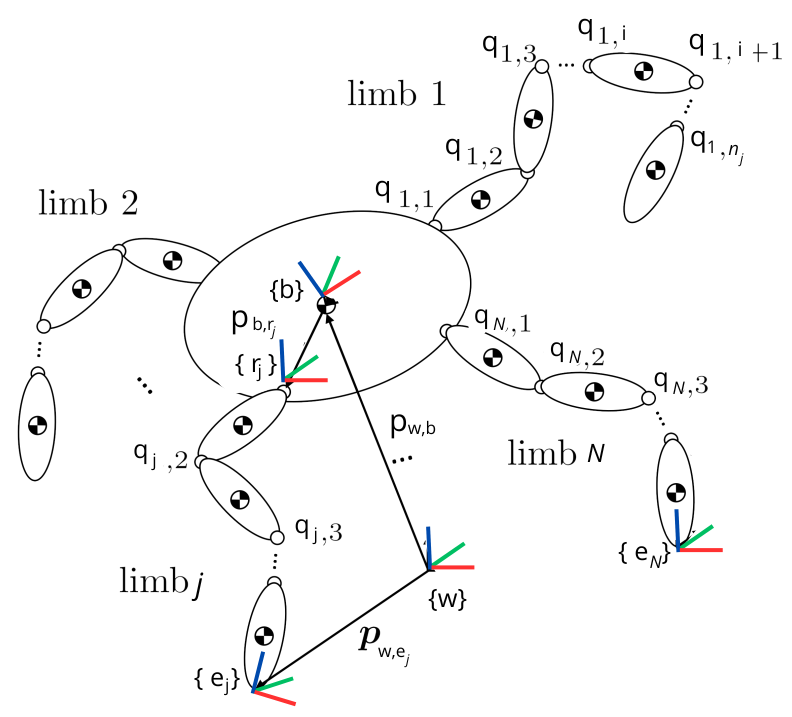
\includegraphics[width=0.35\textwidth]{Images/MultiLimbKin.png}
    \caption{model of multi-limb robot.}
    \label{fig:multilimb}
\end{figure}

An additional kinematic problem, which is relevant when base positioning tasks are considered, is the derivation of the base pose $\mathbf{T^w_b}$ from the limbs configuration, considering the foot pose known in $\mathbf{w}$.

While FK always has a unique solution and standard techniques to solve it, IK is complex, and zero, multiple, or infinite solutions are possible. 

\subsection{Differential Kinematics}
\label{subsec:diff_kin}

The derivation of differential kinematics relation is possible by FK differentiation, but in this research, an alternative approach is considered. 
A multiarm-multilimbed parallelism is considered, 
noticing the following similarities: 
\begin{itemize}
\setlength\itemsep{-0.7pt}
    \item robot base $\leftrightarrow$ manipulated object
    \item $j^{th}$ contact limb $\leftrightarrow$ $j^{th}$ arm
    \item $j^{th}$ limb-end $\leftrightarrow$ $j^{th}$ arm base
    \item $j^{th}$ limb-root $\leftrightarrow$ $j^{th}$ arm end effector 
\end{itemize}


This modeling approximation is possible when the limb-tip interaction with the ground is considered rigid and without sliding. Under this assumption, as represented in Fig.\ref{fig:diffkin}, the limb-root velocity measured in the limb-end frame is the opposite vector of the limb-end velocity in the limb-root frame:$\mathbf{^{e_j}v_{r_j}} = -\mathbf{^{r_j}v_{e_j}}$. 

From this consideration, it is possible to rely on DK to express limb-end motion in the root frame as a function of limb joint velocity, deriving the Jacobian matrix $\mathbf{{^{r_j}J_j}(q_j)}$. Finally, it is converted as limb root velocity, measured in the base frame.
\begin{equation}
\label{eq:rootDK_baseframe}
 \mathbf{^b v_{r_j}} = -\mathbf{J^b_{r_j}}\mathbf{{^{r_j}J_j}(q_j)}\cdot\mathbf{\dot{q}_j} = \mathbf{^b J_j(q_j)}\cdot\mathbf{\dot{q}_j}
\end{equation}

\begin{figure}[H]
    \centering
    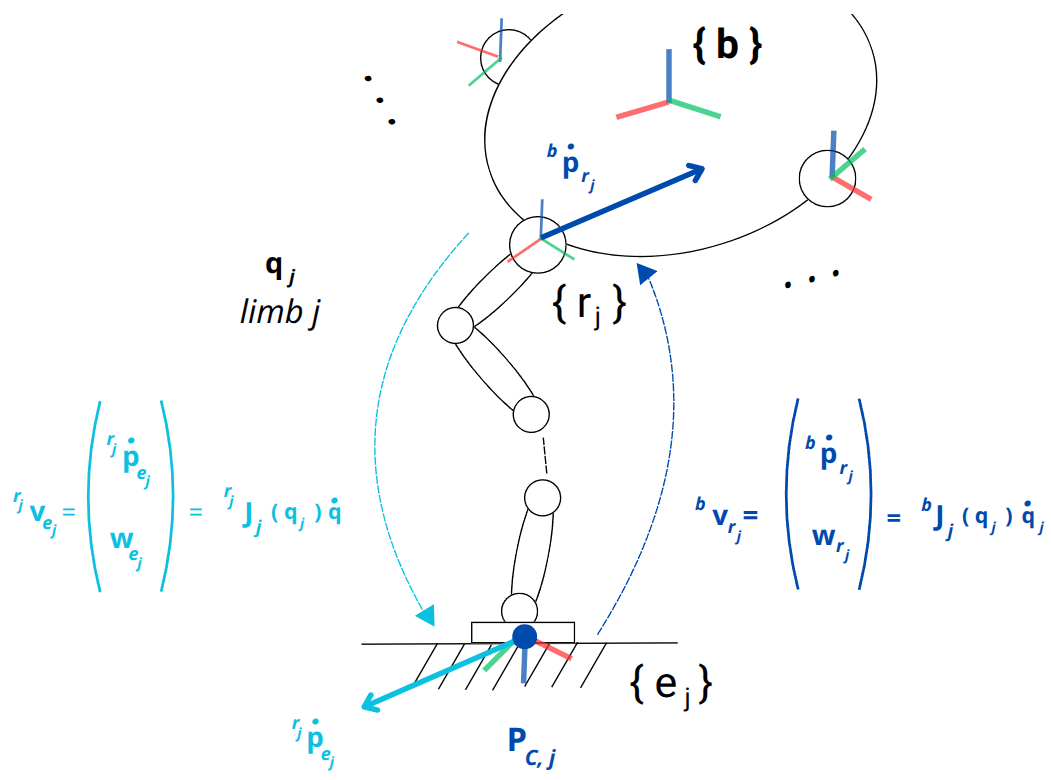
\includegraphics[width=0.35\textwidth]{Images/diffkin_multilimb.png}
    \caption{differential kinematic.}
    \label{fig:diffkin}
\end{figure}

At this point, the single limb is considered as a cooperative manipulator moving the robot base \cite{CooperativeManipulators}\cite{MultiArmManipulability}.
The grasping matrix $\mathbf{W} \in \mathbb{R}^{m \times M}$  ($M = N_c \cdot m$) is defined to relate limb root kinematic with base motion, and the jacobians of the contact limbs are collected in a diagonal matrix. Finally,s the jacobian $\mathbf{J}^T_a(\mathbf{q}) = \mathbf{J}^T(\mathbf{q})\mathbf{W}^\dag \in \mathbb{R}^{n\times m}$  is defined. 
At this point, the absolute velocity of the robot base is computed as: 
\begin{equation}
    \mathbf{v}_a = \mathbf{J}_a(\mathbf{q})\mathbf{\dot{q}}
    \label{eq:MultiLimbvel}
\end{equation}
For the kinetostatic duality\cite{Siciliano}, the relation of statics is is: 
\begin{equation}
    \mathbf{\tau} = \mathbf{J}^T_a(\mathbf{q})\mathbf{h}_a
    \label{eq:MultiLimbKinetostatic}
\end{equation}
Where $\mathbf{h}_a$ denotes the external generalized forces acting on the robot base due to limb interaction.

\subsection{Dynamics}

When a non-minimal number of DOF is used and the floating base DOFs model is employed,$\mathbf{q}=\begin{bmatrix}
    \mathbf{q_b} & \mathbf{q_1} & \mathbf{q_2} & \dots & \mathbf{q_N}
\end{bmatrix}^T$) it is possible to derive the EoM in a standard form with the Lagrange equations:

\label{subsec:dyn}

\begin{subequations}
    \begin{align*}
           \mathbf{B}(\mathbf{q})\mathbf{\ddot{q}} + \mathbf{C}(\mathbf{q},\mathbf{\dot{q}})\mathbf{\dot{q}}+ \mathbf{g}(\mathbf{q}) = \mathbf{J_M}^T(\mathbf{q})\mathbf{\tau} - \mathbf{J_C}^T(\mathbf{q})\mathbf{h_c} \label{eq:WalkingEoM} \\
    \mathbf{J_c}\ddot{\mathbf{q}} + \mathbf{\dot{J}_c}\dot{\mathbf{q}} = 0
    \end{align*}
\end{subequations}


Where the second equation represents the holonomic contact constraint of null velocity at contact point $\mathbf{v_c} = \mathbf{J_c}(\mathbf{q})\mathbf{\dot{q}} = \mathbf{0}$, and 
the matrices involved include the self and coupling effects of all leg joints and base DOF. The matrix $\mathbf{J_M}$ maps all leg joint torques in the space of generalized coordinates. The additional contribution of $\mathbf{\tau_c} = \mathbf{J_c}^T(\mathbf{q})\mathbf{h_c}$ is subtracted at the left-hand side of the EoM to integrate force $\mathbf{h_c}$ applied at a generic point $\mathbf{C}$ in the structure (such as contact forces).

When the system is quasi-static and complex whole-body dynamics can be approximated, the single limb is analyzed singularly with the reduced order robotic arm dynamic model\cite{Siciliano}. 

\subsection{Control}
\label{subsec:control}

The control of multilimbed robots is possible using multilayered control structures, composed of high-level, middle-level, and low-level components, with additional global planners and state estimators. 
Part of the state estimators are mapping and terrain traversability estimation, but also internal robot state and contact point understanding. Global planners are responsible for sending high-level tasks to the layered control structure, where the task is received by the high-level controller.At this point, a chained computation and transformation from high to low-level commands occur in the layered control structure, until hardware commands are sent to the robot. Many different control strategies can be integrated simultaneously in this layered structure, such as Model Predictive Control, Whole Body Controller, Model Free Reinforcement learning policies, Torque-based control, or simpler Inverse kinematic independent joint controllers. 


%-----------------------------------------------------------------------------
% MODELING CONTROL AND ANALYSIS
%-----------------------------------------------------------------------------
\section{Stability and Performance of Multilimbed Robots}
\label{sec:multilimb_performance}

\subsection{Stability}
\label{subsec:stability}

Stabilizing machines with discontinuous contact points during locomotion has been addressed by many researchers\cite{LeggedStability}, and different theories exist. 

Defining the support polygon (SP) as the convex hull formed by the contact points of the feet in the support plane ($\mathbf{P}_{c,j},\forall j \in J_c$), static stability is ensured if the base CoM projection $\overline{\mathbf{P}_{CoM}}$ on the ground is contained inside the SP. 
From these requirements, stability margins are derived (represented in Fig.\ref{fig:stability}), with the \textbf{SSM} defining the smallest distance between $\overline{\mathbf{P}_{CoM}}$ and the SP perimeter ($\partial SP$). 

\begin{figure}[H]
    \centering
    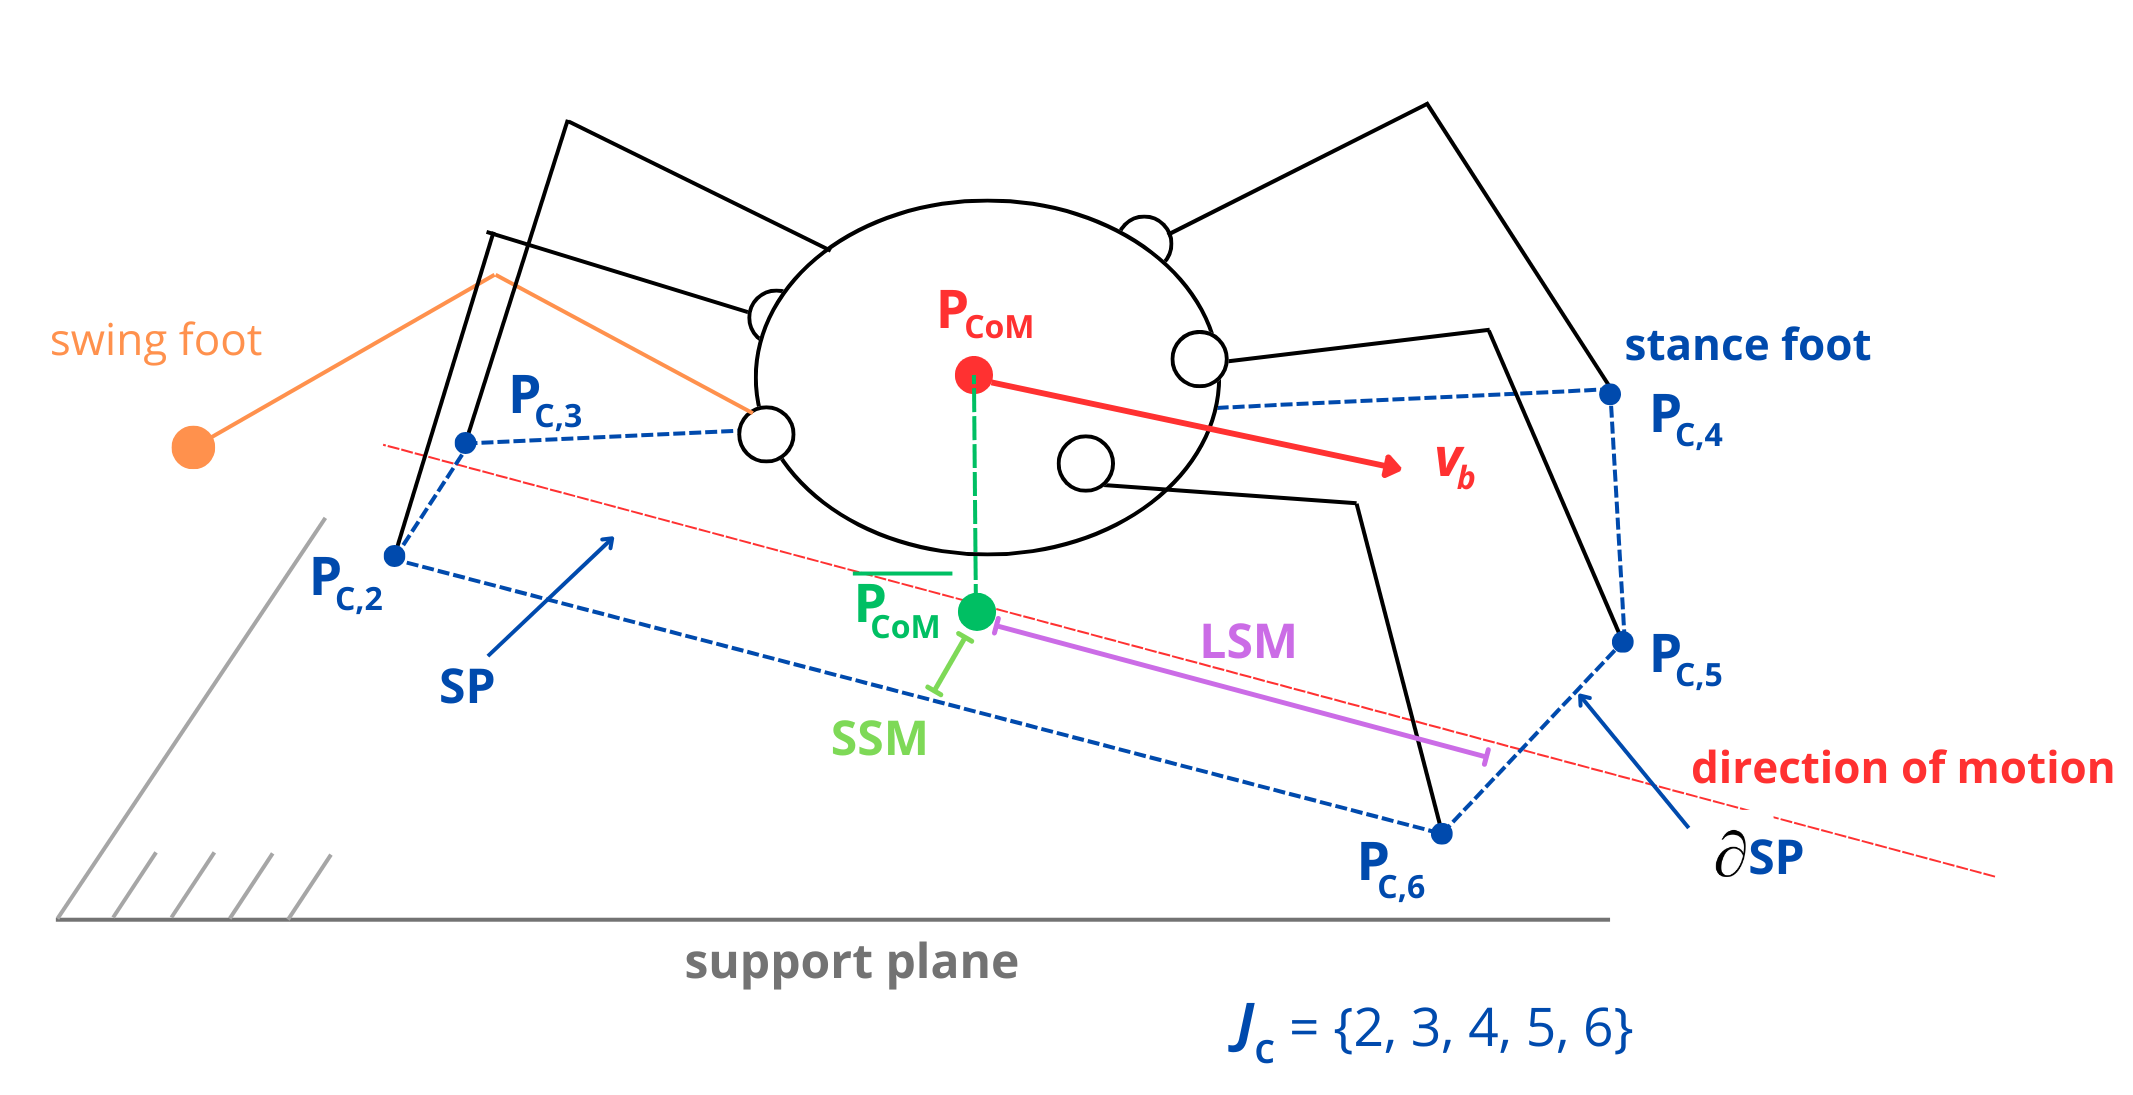
\includegraphics[width=0.35\textwidth]{Images/StabilityMargin1.png}
    \caption{Stability analysis on flat terrains.}
    \label{fig:stability}
\end{figure}

For this research, the problem of motion during transformation is addressed, and it is assumed that this task occurs on a flat surface with negligible inertia effects, where $SSM > 0$ ensures system stability. 
To define an absolute index for comparable results independent of robot dimensions, a normalized percentage SSM has been defined as
\begin{equation}
\label{eq:SSMpercentage}
    SSM_\% = \frac{SSM}{SSM_{max}}\cdot100
\end{equation}
Where the $SSM_{max}$ corresponds to the maximum relative stability margin measured in meters (when the robot is on 4 contact points on a standard walking configuration).

When rough terrains or stability with gripping forces has to be analyzed, other criteria exist, such as the Zero Moment Point, tumble stability, and Gravito Inertia Acceleration (GIA)\cite{GIA_polyedron}

\begin{figure*}[t]
    \centering
    \subfloat[Grasshopper jumping Manipulability analysis.\label{fig:ellipsoidGrasshopper}]{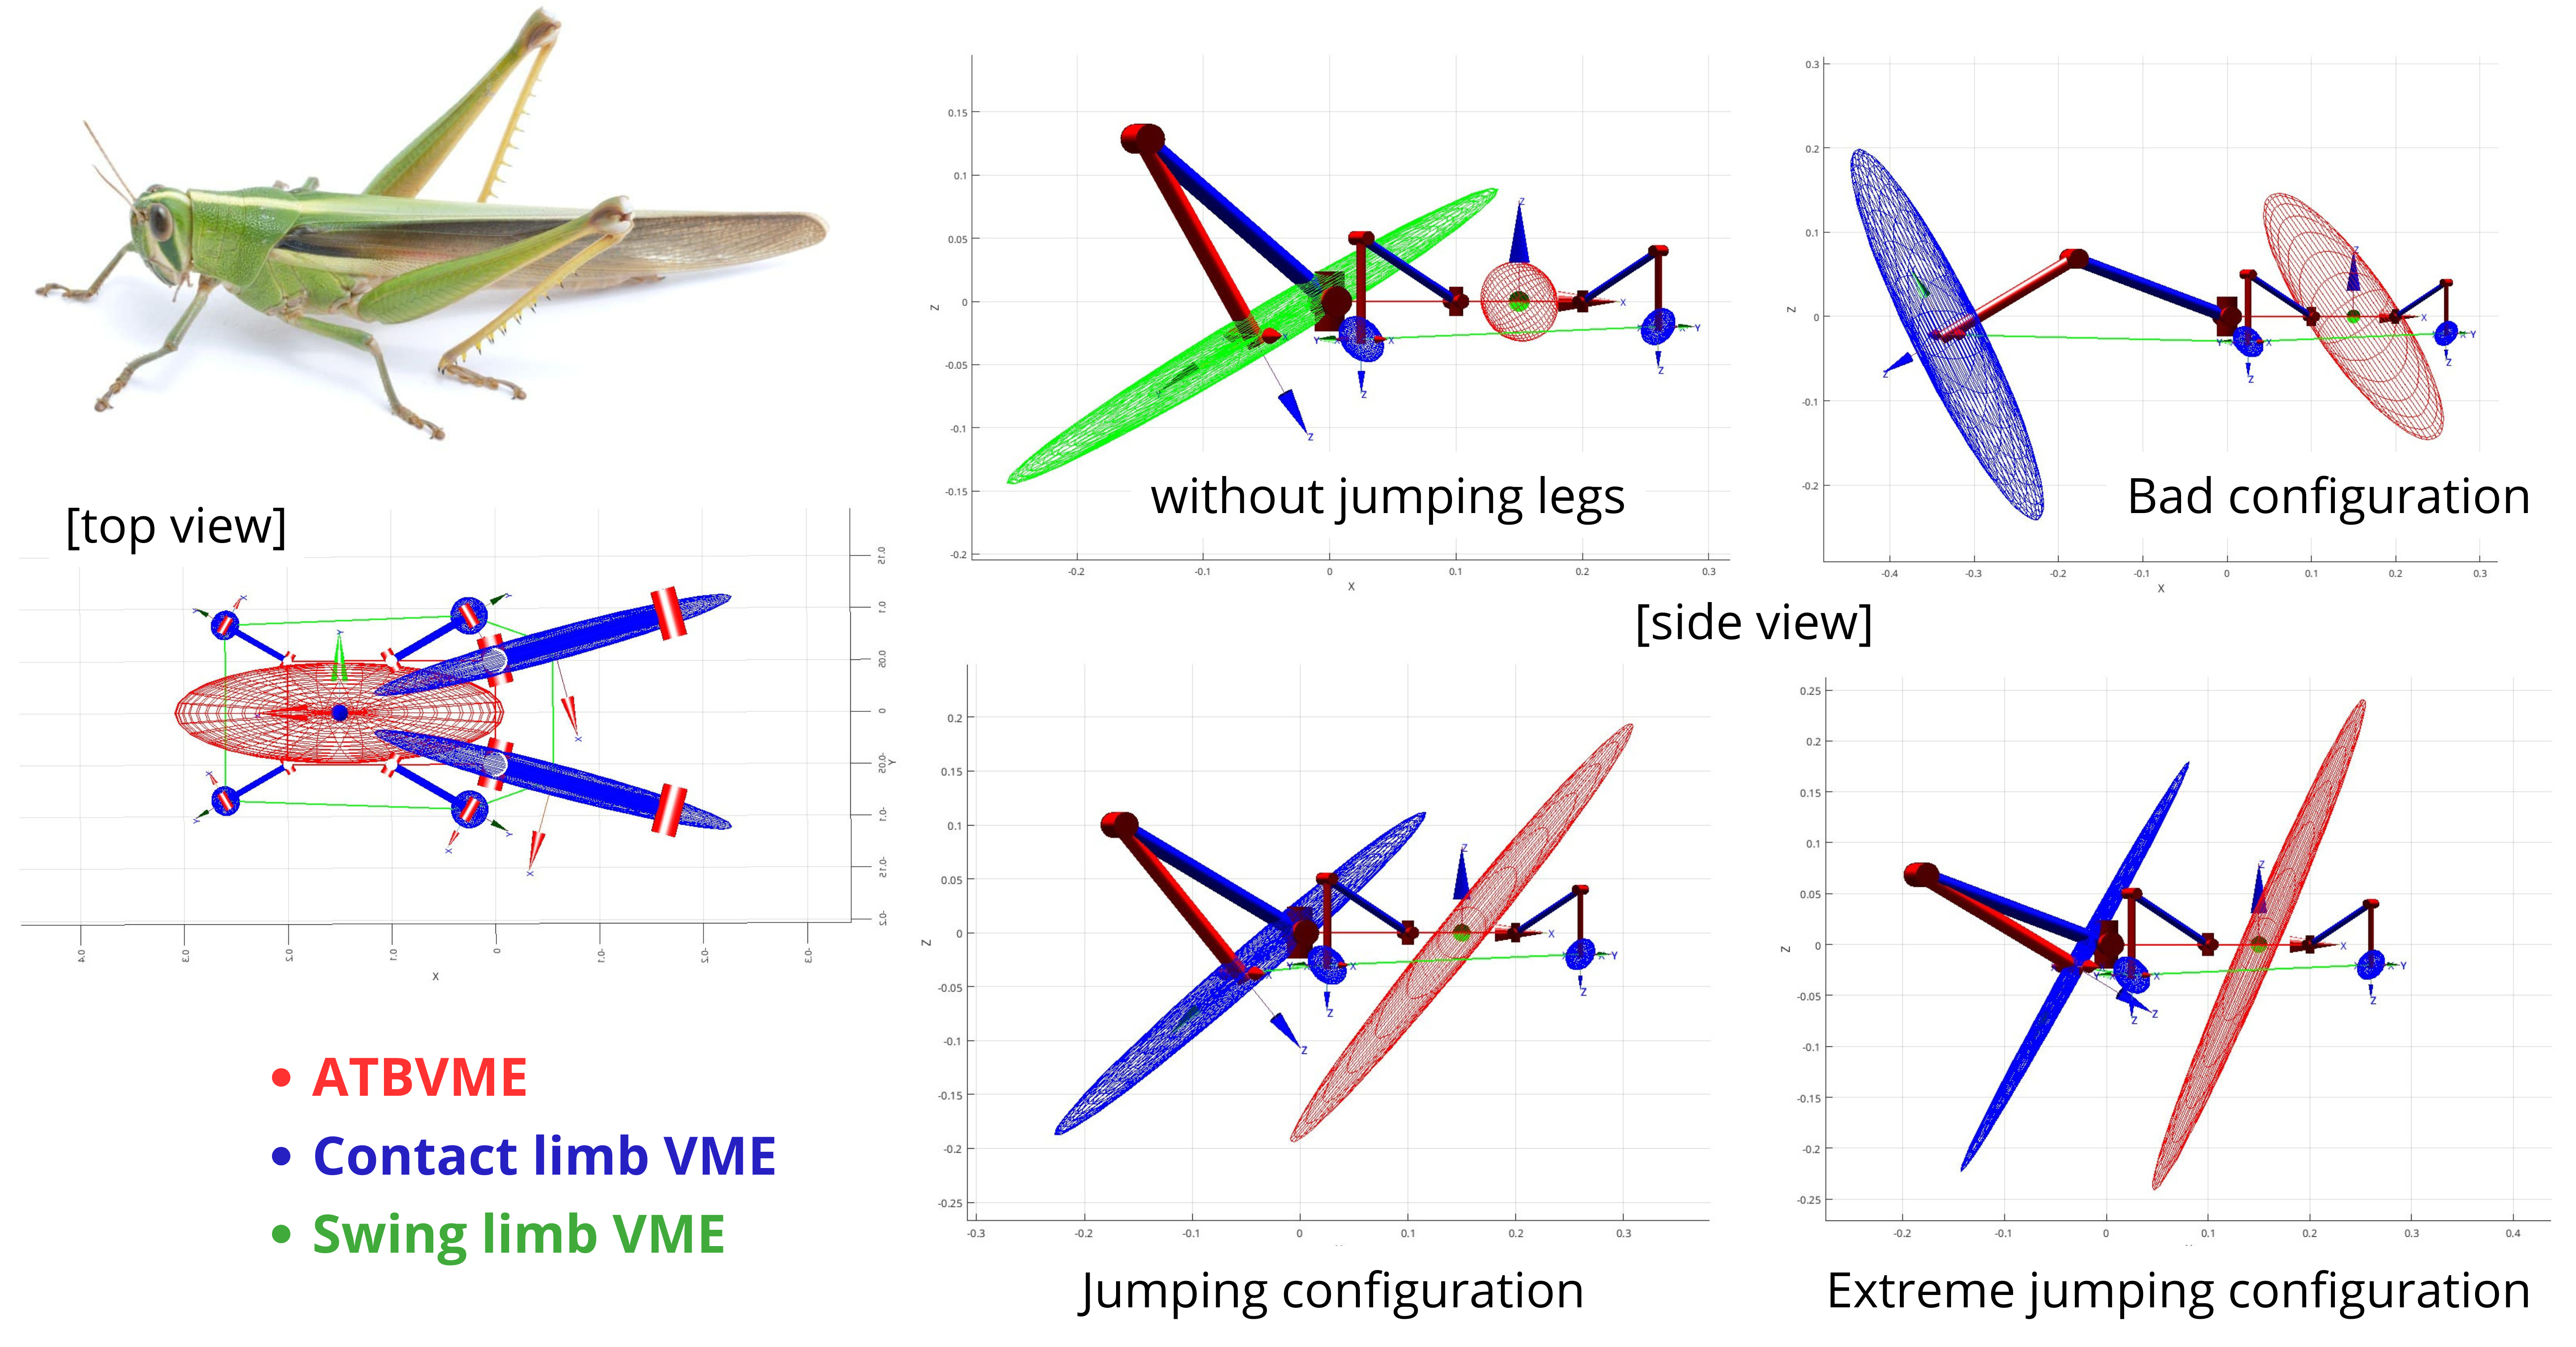
\includegraphics[width=0.5\textwidth]{Images/grasshopper_ellipsoid.png}}
    \subfloat[4-limbed and 6-limbed robot manipulability.\label{fig:ellipsoidQuadruped}]{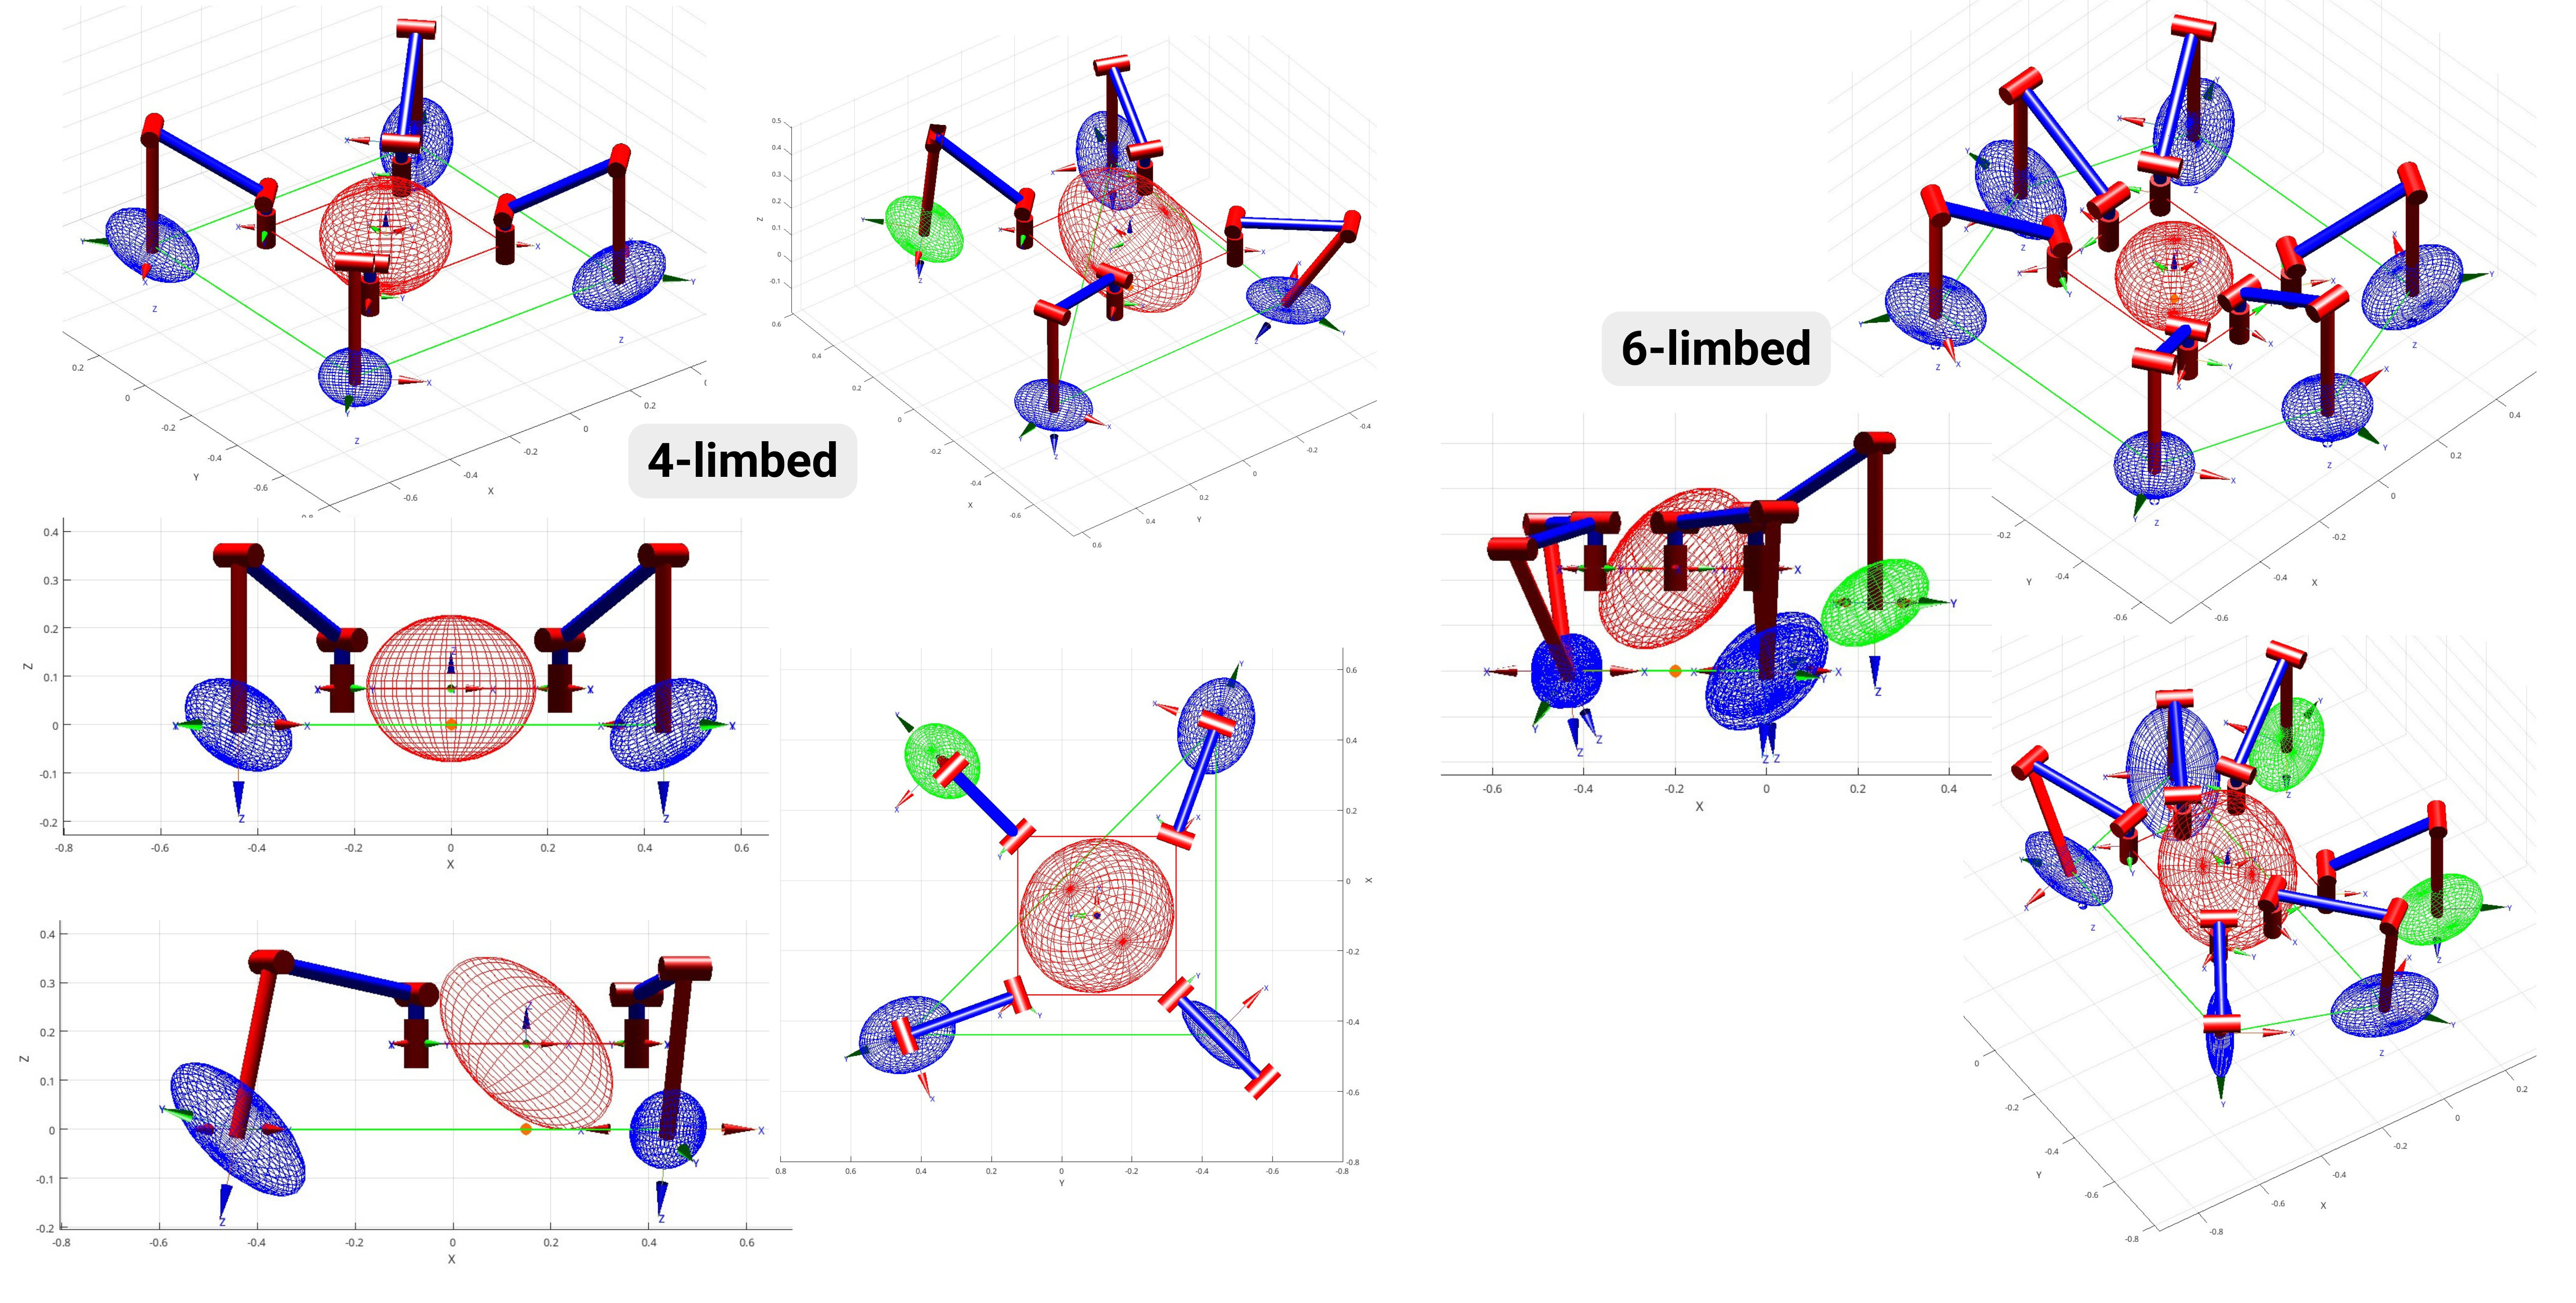
\includegraphics[width=0.5\textwidth]{Images/Quadruped_ellipsoid.png}} 
    \caption{ATBVME Dexterity analysis of multilimbed systems (bio-inspired and robotics)}
    \label{fig:ATBVME}
\end{figure*}

\subsection{Manipulability}
\label{subsec:manipulability}

The manipulability theory first introduced by T.Yoshikawa\cite{ManipulabilityYoshikawa} defines the manipulability ellipsoid (in velocity or force) as the mapping of a hyper-spherical joint-space domain in the task space: 
\begin{equation}
\label{eq:EllipsoidVel}
    \mathbf{\dot{q}}^T \mathbf{\dot{q}} = \mathbf{v_f}(\mathbf{J}\mathbf{J}^T)^{-1}\mathbf{v_f} = 1
\end{equation}
\begin{equation}
\label{eq:EllipsoidForce}
    \mathbf{\tau}^T \mathbf{\tau} = \mathbf{h_f}^T(\mathbf{J}\mathbf{J}^T)\mathbf{h_f} = 1
\end{equation}

In this work, the cooperative manipulator manipulability theory \cite{MultiArmManipulability} has been extended for multilimbed robots, deriving the base manipulability ellipsoid (BME) for limbed robots. This is possible due to the duality discussed previously, for which the multi-limb robot is modeled as a system of cooperative manipulators, with the proper modeling considerations. 

From relation (\ref{eq:MultiLimbvel}) and (\ref{eq:MultiLimbKinetostatic}) the \textit{\textbf{external base force manipulabnility ellipsoid}} for the base (EBFME), and the \textit{\textbf{absolute base velocity manipulability ellipsoid}} (ABVME) are defined as follows: 
\begin{equation}
    \mathbf{h}^T_a [\mathbf{J}_a(\mathbf{q})\mathbf{J}^T_a(\mathbf{q})]\mathbf{h}_a = 1
    \label{eq:BEFME}
\end{equation}
\begin{equation}
    \mathbf{v}^T_a [\mathbf{J}_a(\mathbf{q})\mathbf{J}^T_a(\mathbf{q})]^{-1}\mathbf{v}_a = 1
    \label{eq:ABVME}
\end{equation}

The matrix $\mathbf{E}_a \in \mathbb{R}^{m\times m}$ represents the core of the EBFME's quadratic form, while its inverse is the ABVME's. 
The expression of the ellipsoid matrix can be decomposed as: 
\begin{equation}
\label{eq:BME_decoupled}
    \mathbf{E}_a = \begin{bmatrix}
        \mathbf{E_T}_a & \mathbf{E_{TR}}_a \\
        \mathbf{E^T_{TR}}_a & \mathbf{E_{R}}_a 
    \end{bmatrix}
\end{equation}
Where $\mathbf{E_T}_a \in \mathbb{R}^{m_P \times m_P}$ is the core of the translational BME (TBME),  
$\mathbf{E_R}_a \in \mathbb{R}^{m_O \times m_O}$
is the core of the rotational BME (RBME),
and $\mathbf{E_{TR}}_a \in \mathbb{R}^{m_P \times m_O}$ is a coupling matrix\cite{TRManipulability}.

The results of the application of the ATBVME on a bio-inspired example of a grasshopper jump is reported in Fig.\ref{fig:ellipsoidGrasshopper}, while Fig.\ref{fig:ellipsoidQuadruped} analyze a 4-limbed and 6-limbed simple robot. 

%-----------------------------------------------------------------------------
% LIMBERO-GRIEEL
%-----------------------------------------------------------------------------
\section{LIMBERO-GRIEEL}
\label{sec:limbero_grieel}

\textbf{LIMBERO} (\textbf{LIMB}-climbing \textbf{E}xploration \textbf{RO}bot) is a prototype omnidirectional four-limbed robot\cite{LIMBEROTakadaThesis}, designed, 3D printed, and assembled by the Limb Team at the Space Robotics Lab. It is a small lightweight climbing robot, with a claw-type gripper\cite{KentaroUnoPhD} in its default design.\\
\textbf{GRIEEL} (\textbf{GRI}pper wh\textbf{EEL}) is a prototype gripper-wheel transformable mechanism, designed and patented by Masahiro Uda \textit{et all}\cite{GrieelUda}\cite{GRIEELUdaThesis}, member of the SRL Rover Team.  

\textbf{LIMEBRO-GRIEEL} is obtained from the assembly of the two systems described above, enabling wheeled locomotion in addition to walking and climbing. The limb structure is represented in Fig.\ref{fig:limb_dofs}, while the different modalities are reported in Fig.\ref{fig:transform}.

The motion controller and the planner respect the multilayered structure previously defined and are implemented with an articulated ROS2 architecture\cite{ROS2}.
For this research, different implementations of the motion controller have been considered, all with a position-based IK independent joint controller. In particular, a ready-to-use joint trajectory controller (JTC) (coming from the ros2\_control framework) has been used in the preliminary simulation testing. The DYNAMIXELs servomotors' internal PID is used with the real system (DYCs). Finally, a custom independent joint cascade PPI controller is used with a different simulation configuration (IJCs). 

\begin{figure*}[t]
    \centering
    \subfloat[Limb model, DOFs.\label{fig:limb_dofs}]{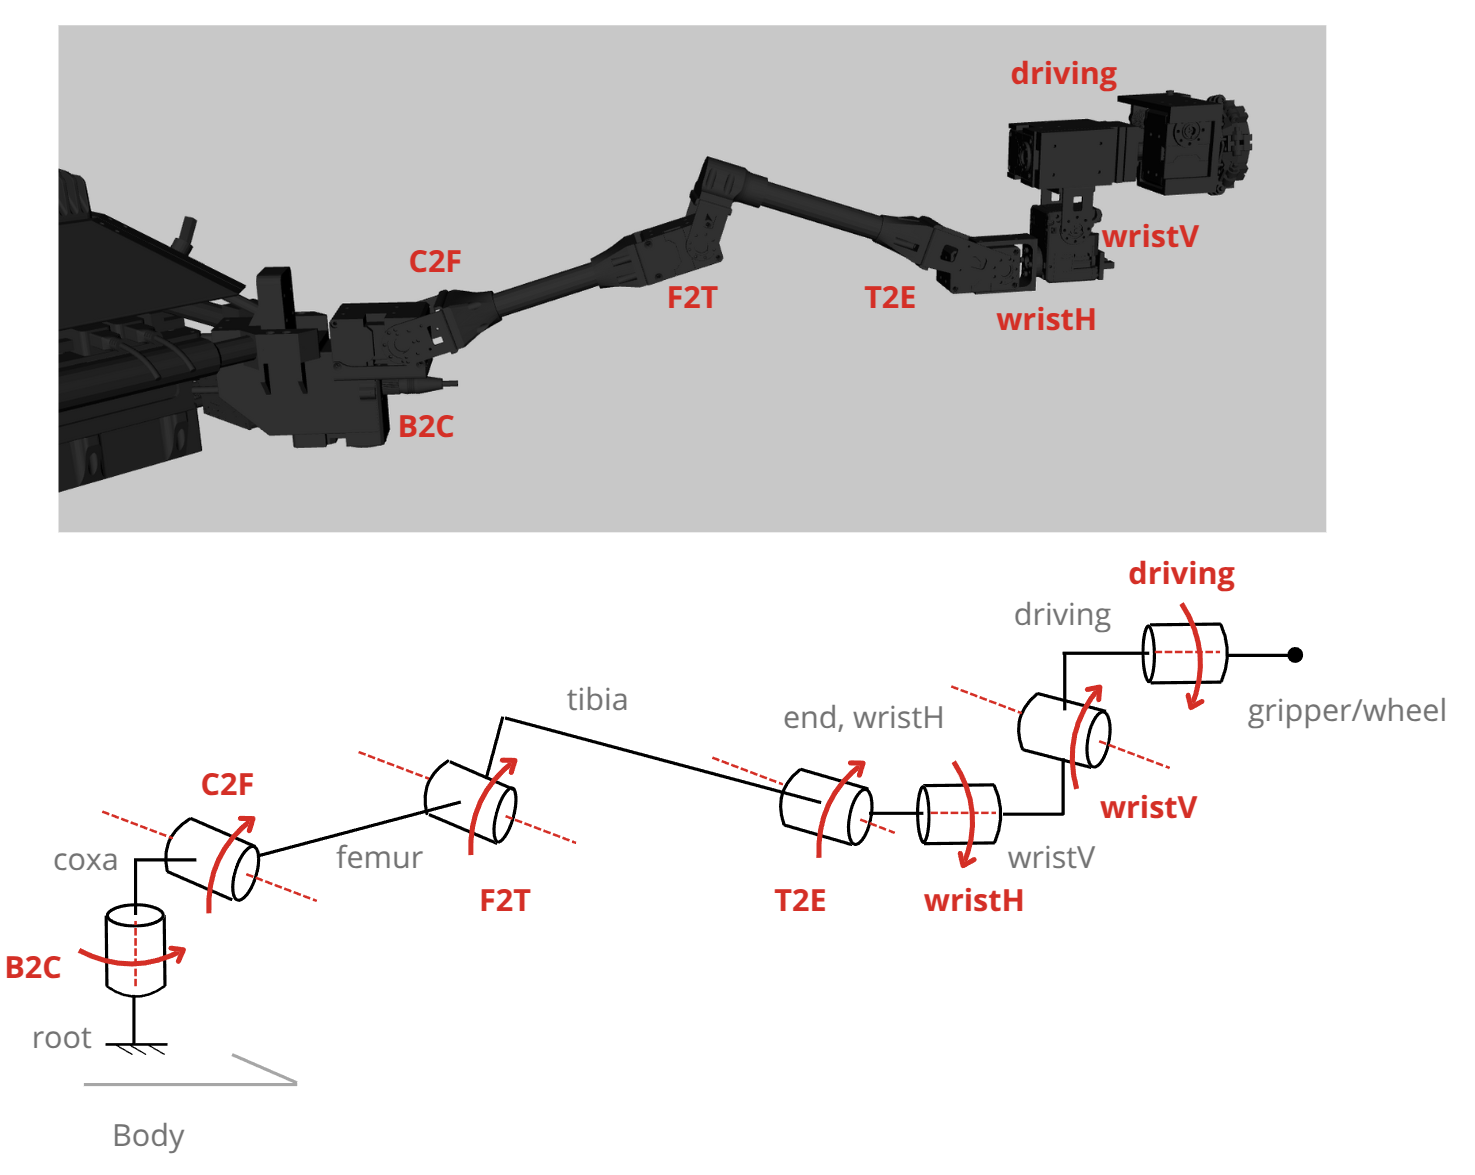
\includegraphics[width=0.4\textwidth]{Images/LIMBERO_GRIEEL_limb_model.png}}
    \subfloat[Wheel and Gripper Mode transition.\label{fig:transform}]{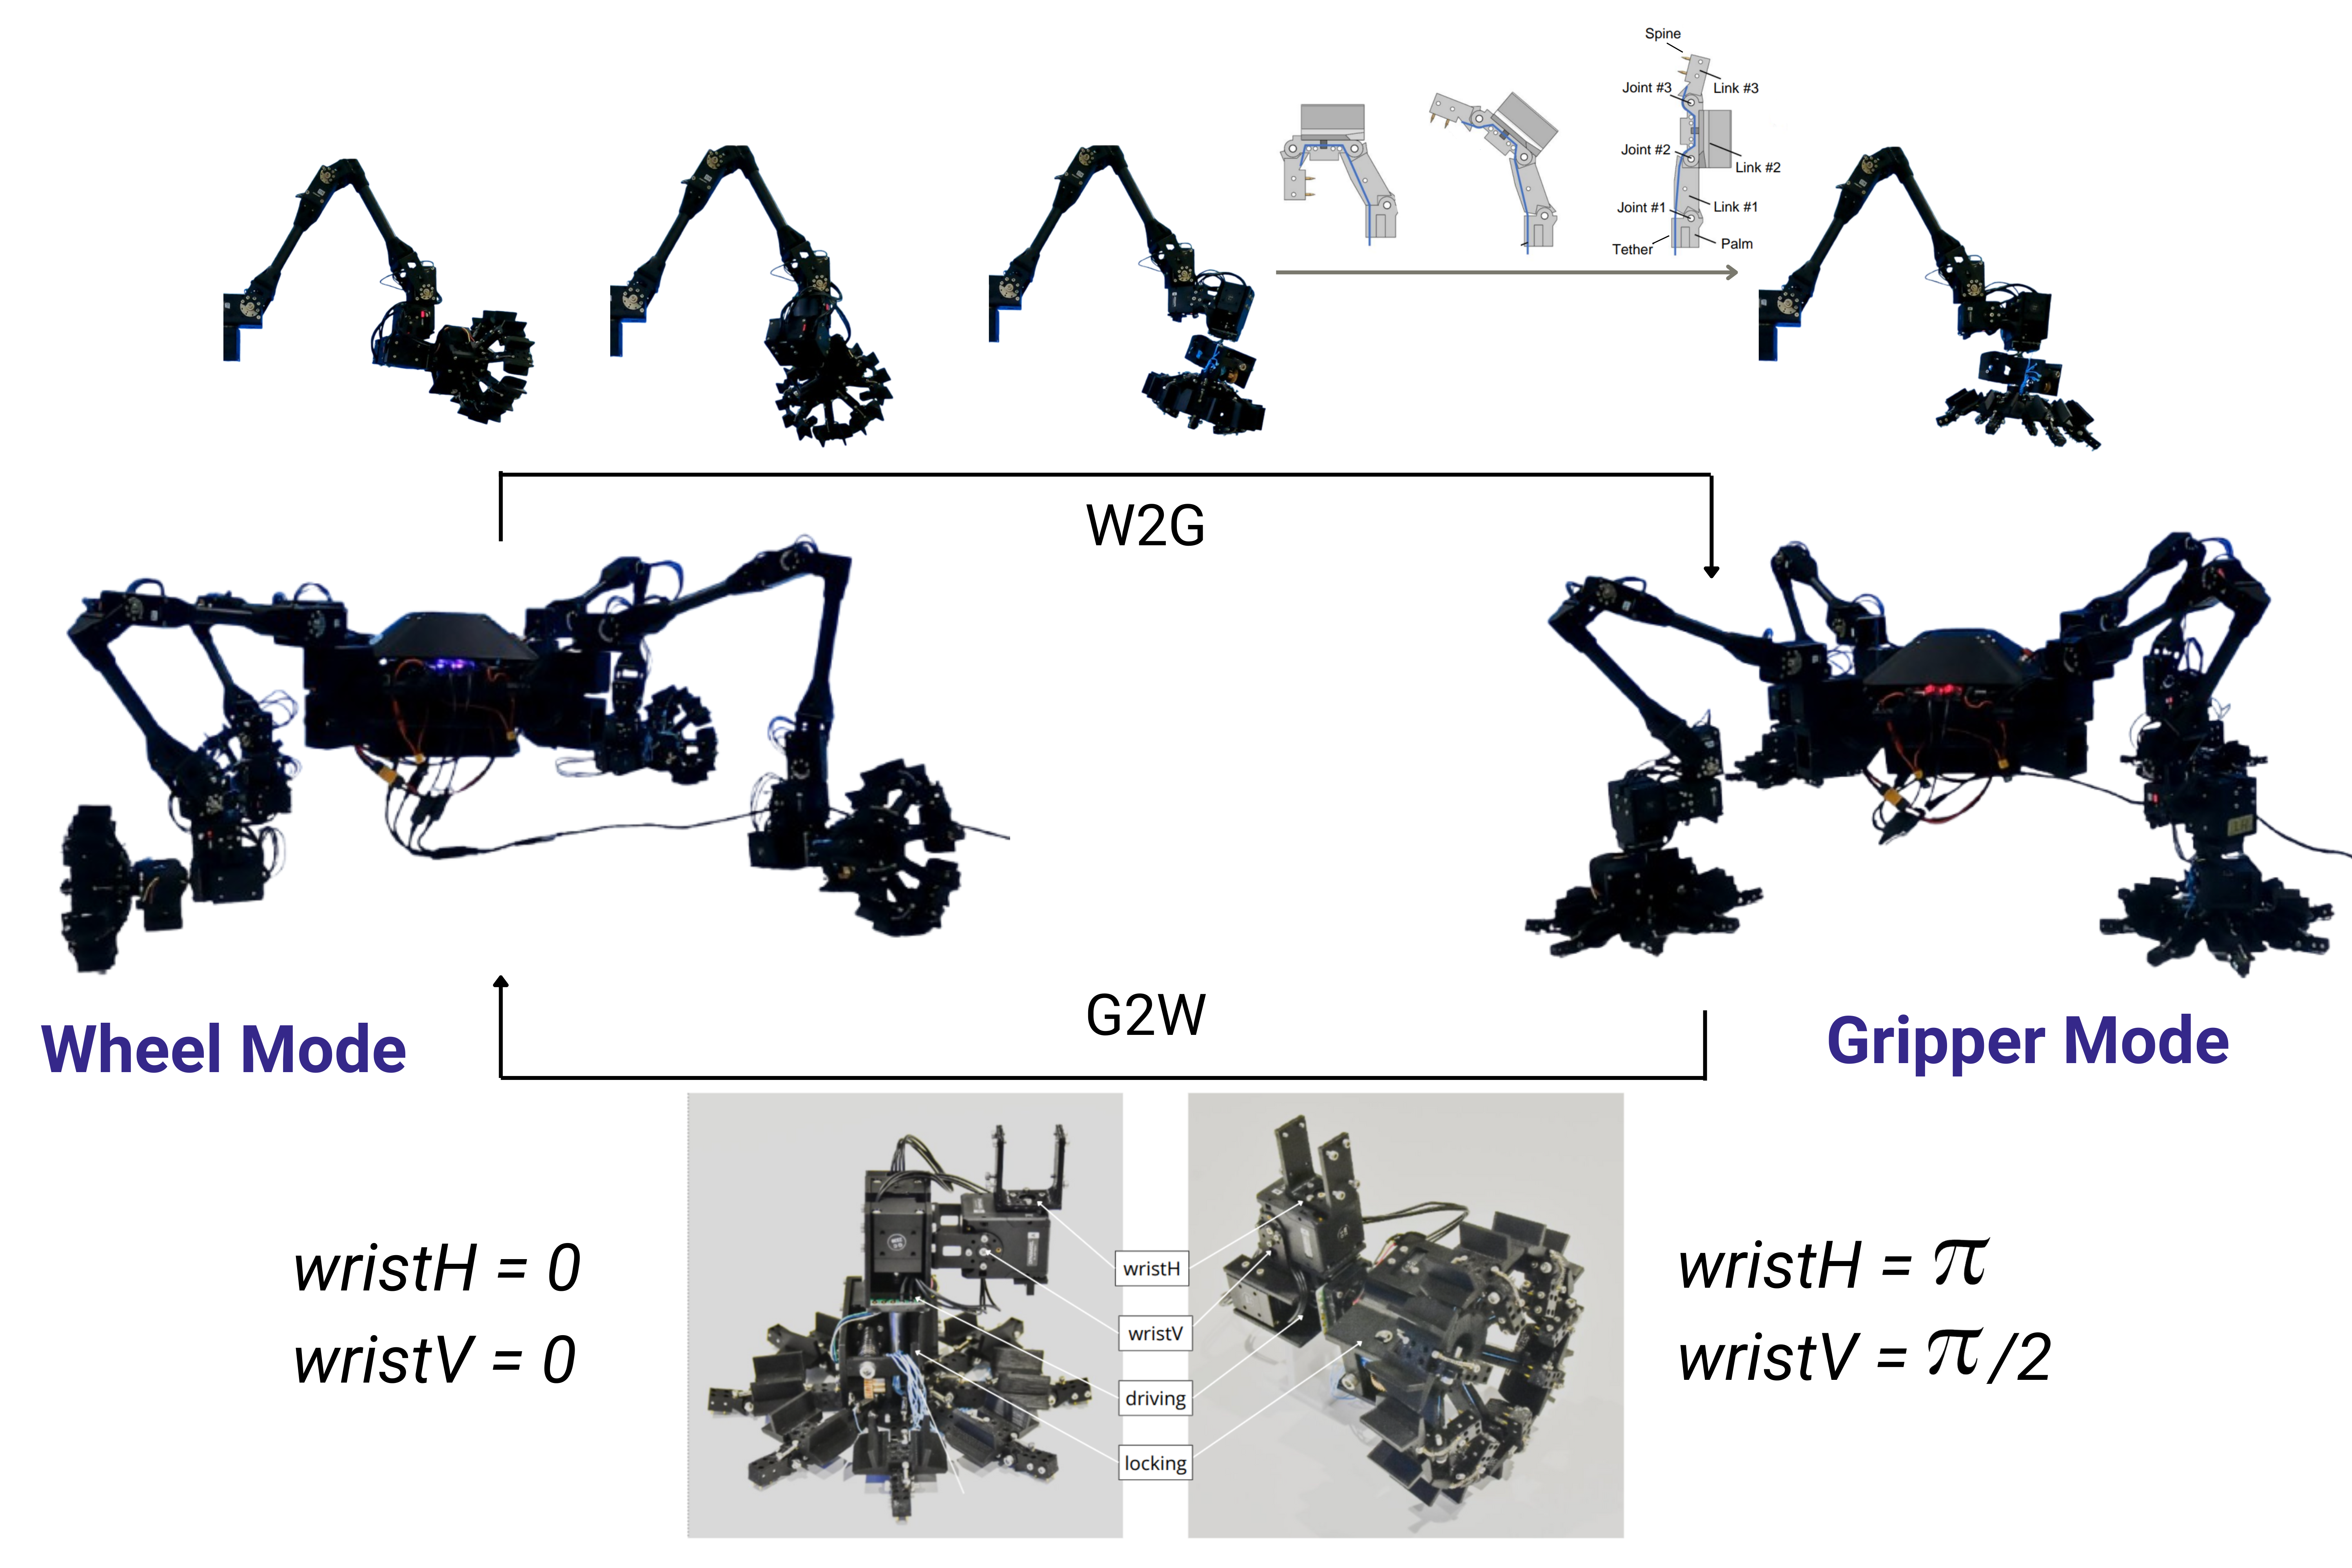
\includegraphics[width=0.6\textwidth]{Images/LIMBERO_GRIEEL.png}} 
    \caption{LIMBERO-GRIEEL, limb model and GRIEEL transition sequence}
    \label{fig:limbero_grieel}
\end{figure*}


%-----------------------------------------------------------------------------
% MODE TRANSITION ALGORITHM
%-----------------------------------------------------------------------------
\section{Mode Transition Algorithm}
\label{sec:multimode_alg}

In the previous work\cite{GRIEELUdaThesis}, the mode transformation was defined with a simple but non-reliable motion sequence, in which the base lay on the ground during simultaneous module transition. In this research, the algorithm to change mode has been designed and implemented with an adaptable sequence that maintains stability and dexterity, sustaining the base above the ground.
This algorithm is summarized in Fig.\ref{fig:algorithm}, and it consists of anticipative planning and motion task execution.

In the proposed algorithm, the transformation is considered as a set of single tasks. First, a future stable base pose is estimated, and then the task is executed as base motion, limb raise, support on three contact points, module transition, and limb down. This singular module transformation makes possible hybrid configurations transition, such as three-wheeled driving with single-limb manipulation. 

\begin{figure}[H]
    \centering
    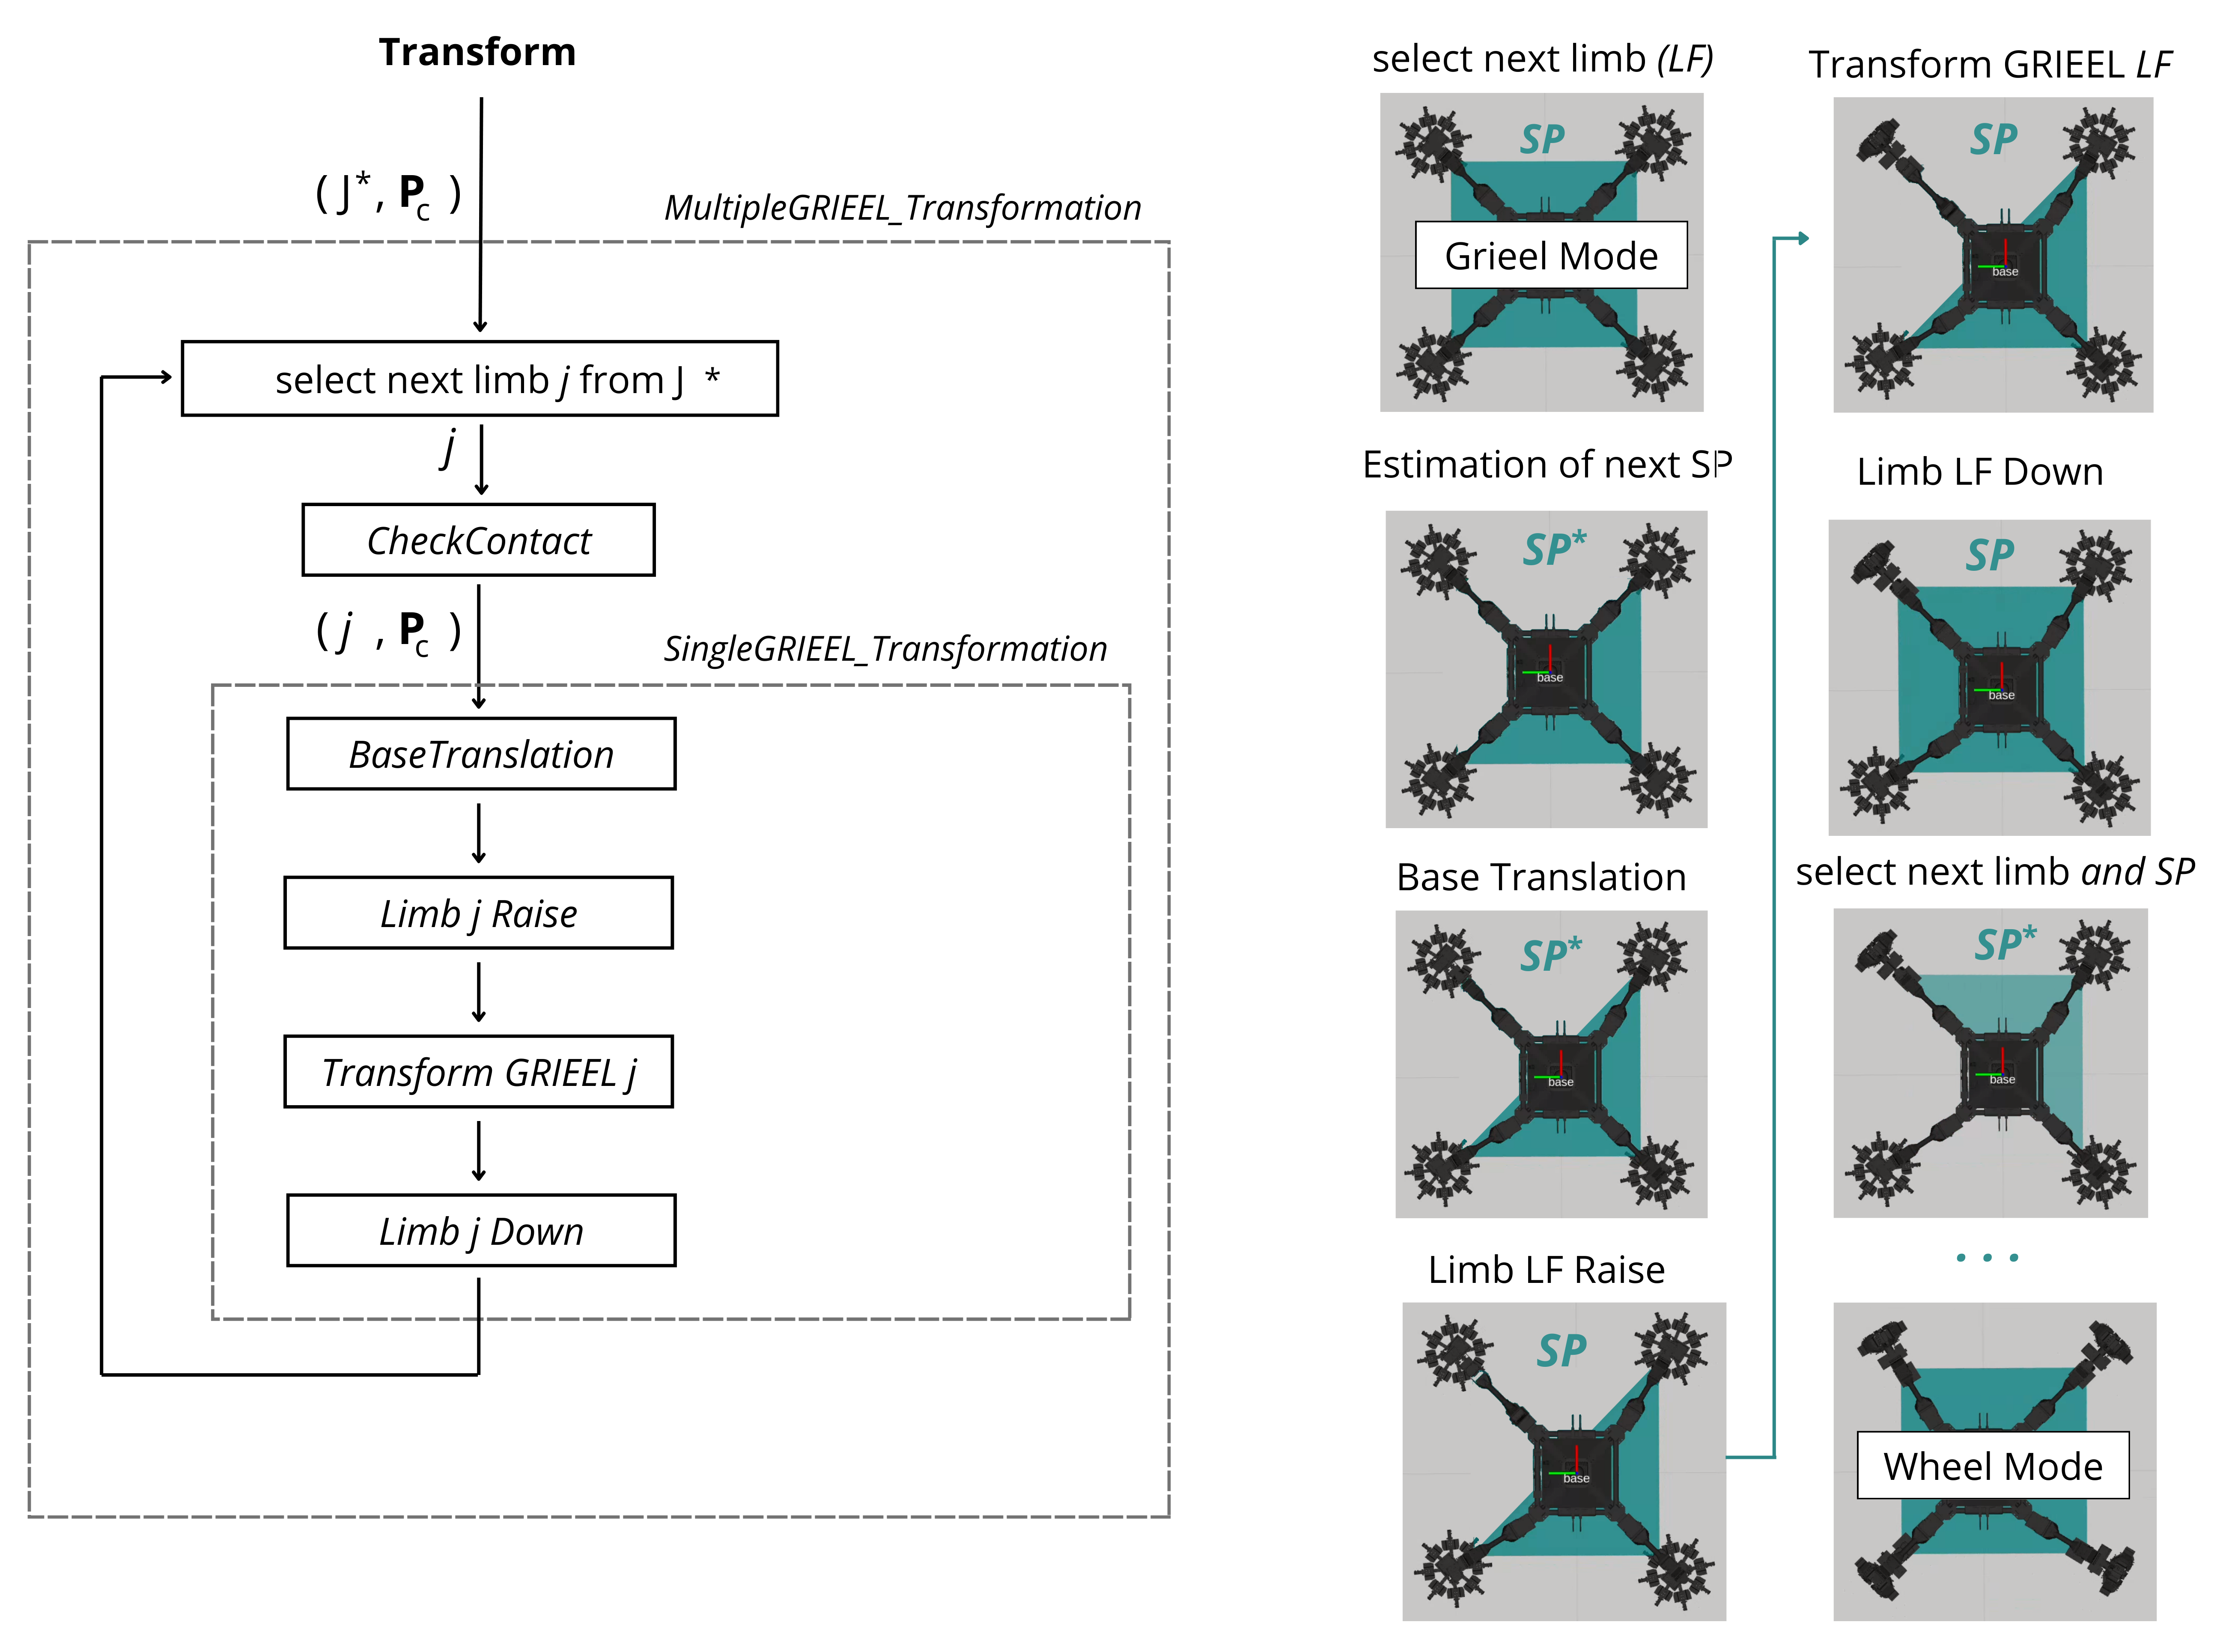
\includegraphics[width=0.40\textwidth]{Images/complete_transition.png}
    \caption{Transformation algorithm.}
    \label{fig:algorithm}
\end{figure}


%-----------------------------------------------------------------------------
% SIMULATIONS AND EXPERIMENTS SETUP
%-----------------------------------------------------------------------------
\section{Simulation and Experiments}
\label{sec:sim}

Different testing environments have been used, with different objectives and control systems implementation. 
\subsection{Motion Controller Tuning}
\label{subsec:tuning}

The JTC, used for preliminary algorithm and communication testing in Gazebo Classic, is configured with an empirical tuning approach. Iterative adjustments with a \textit{root-2-end}, \textit{end-2-root} logic is considered.
From the gains of the JTC, the DYCs gains are adjusted by single limb experiments on the real hardware. Finally, with a more realistic simulation setup in Gazebo Harmonic, a custom closed-loop controller has been implemented, and tuned with a model-based approach, after deriving a limb dynamic model in MATLAB from the simulation description.  

\subsection{Preliminary Simulations}
\label{subsec:sim0}

This initial simulation setup has been fundamental for: 
\begin{itemize}
    \setlength\itemsep{-0.7pt}  
    \item \textbf{Software update}: testing the software to control GRIEEL's joints.
    \item \textbf{Transformation algorithm}: Developing and testing the mode transition algorithm.
    \item \textbf{Reliable physics computation}: Gazebo uses a physics engine that includes forces such as inertial effect, gravity, and friction, providing a realistic environment.
\end{itemize}

\subsection{Experiments}
\label{subsec:exp}

The experimental setup is fundamental to verify if the implemented algorithms and control structure are correctly integrated with the real system. 
In particular, single-limb tests are conducted for safe preliminary experiments. 
Finally, simple tasks and the locomotion transition algorithm are tested on the assembled LIMBERO-GRIEEL robot.  

\begin{figure*}[t]
    \centering
    \subfloat[G2W Experiment results.\label{fig:experimentG2W}]{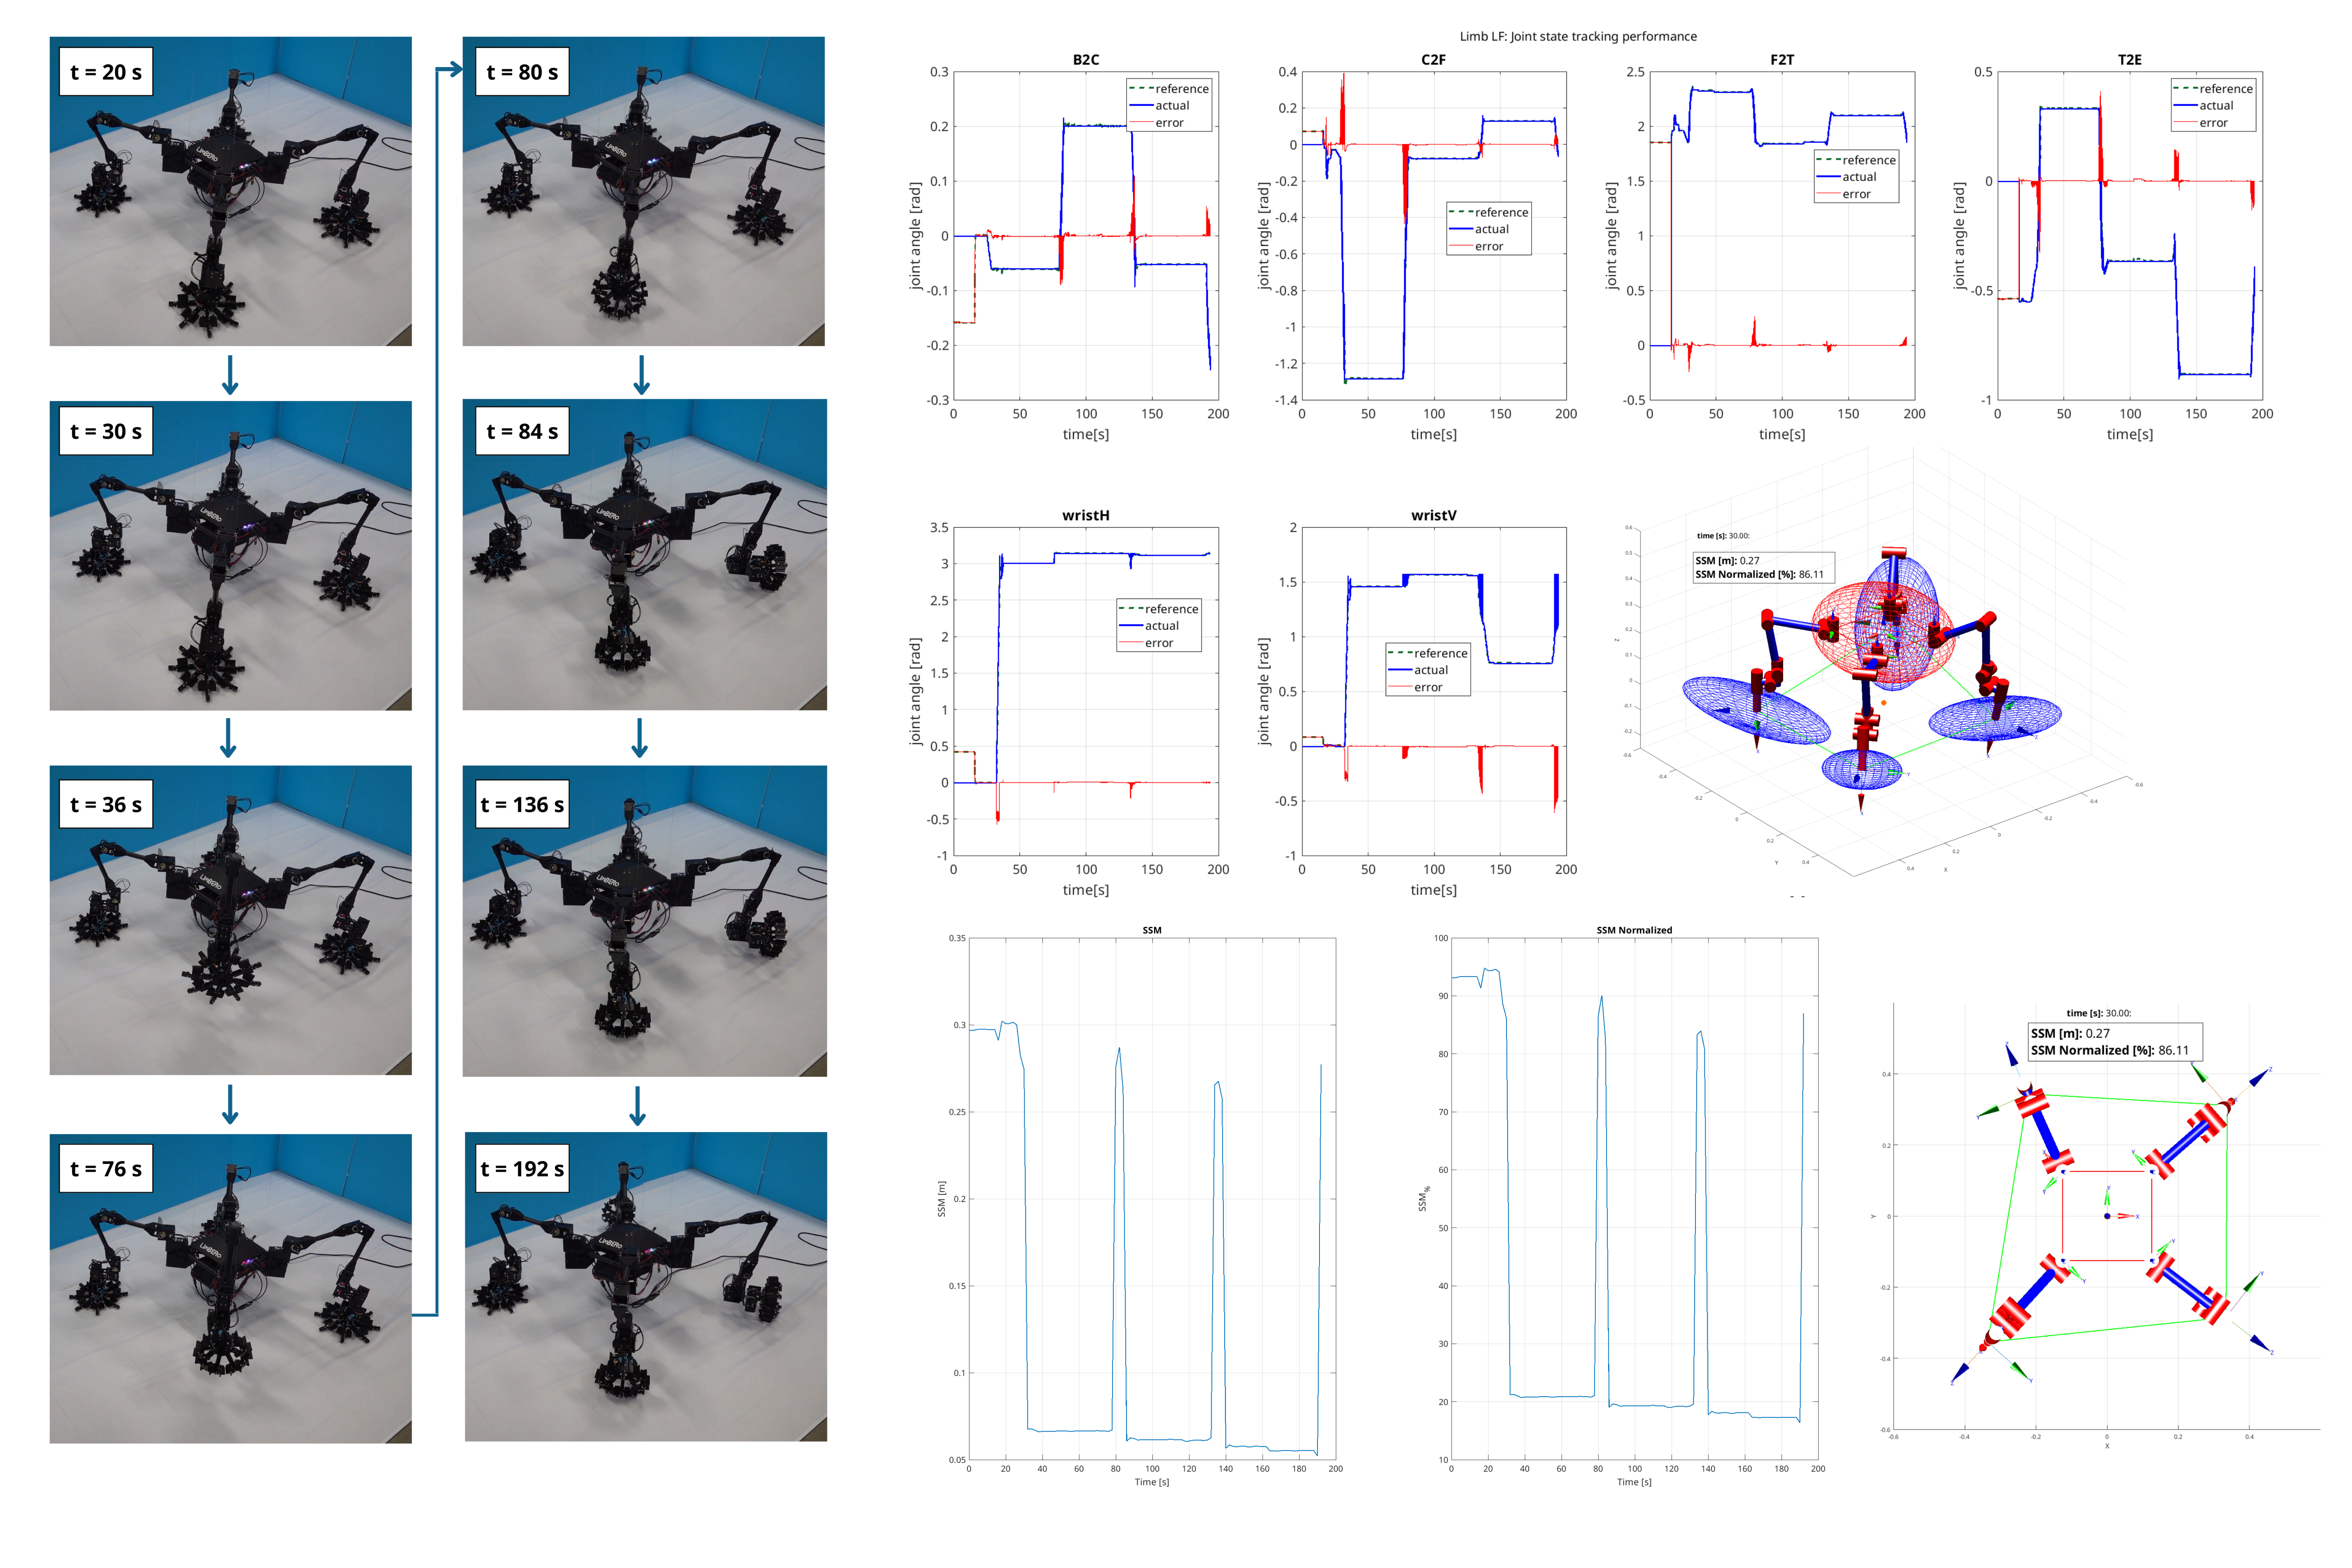
\includegraphics[width=0.5\textwidth]{Images/experiment.png}}
    \subfloat[W2G Simulation results.\label{fig:simulationW2G}]{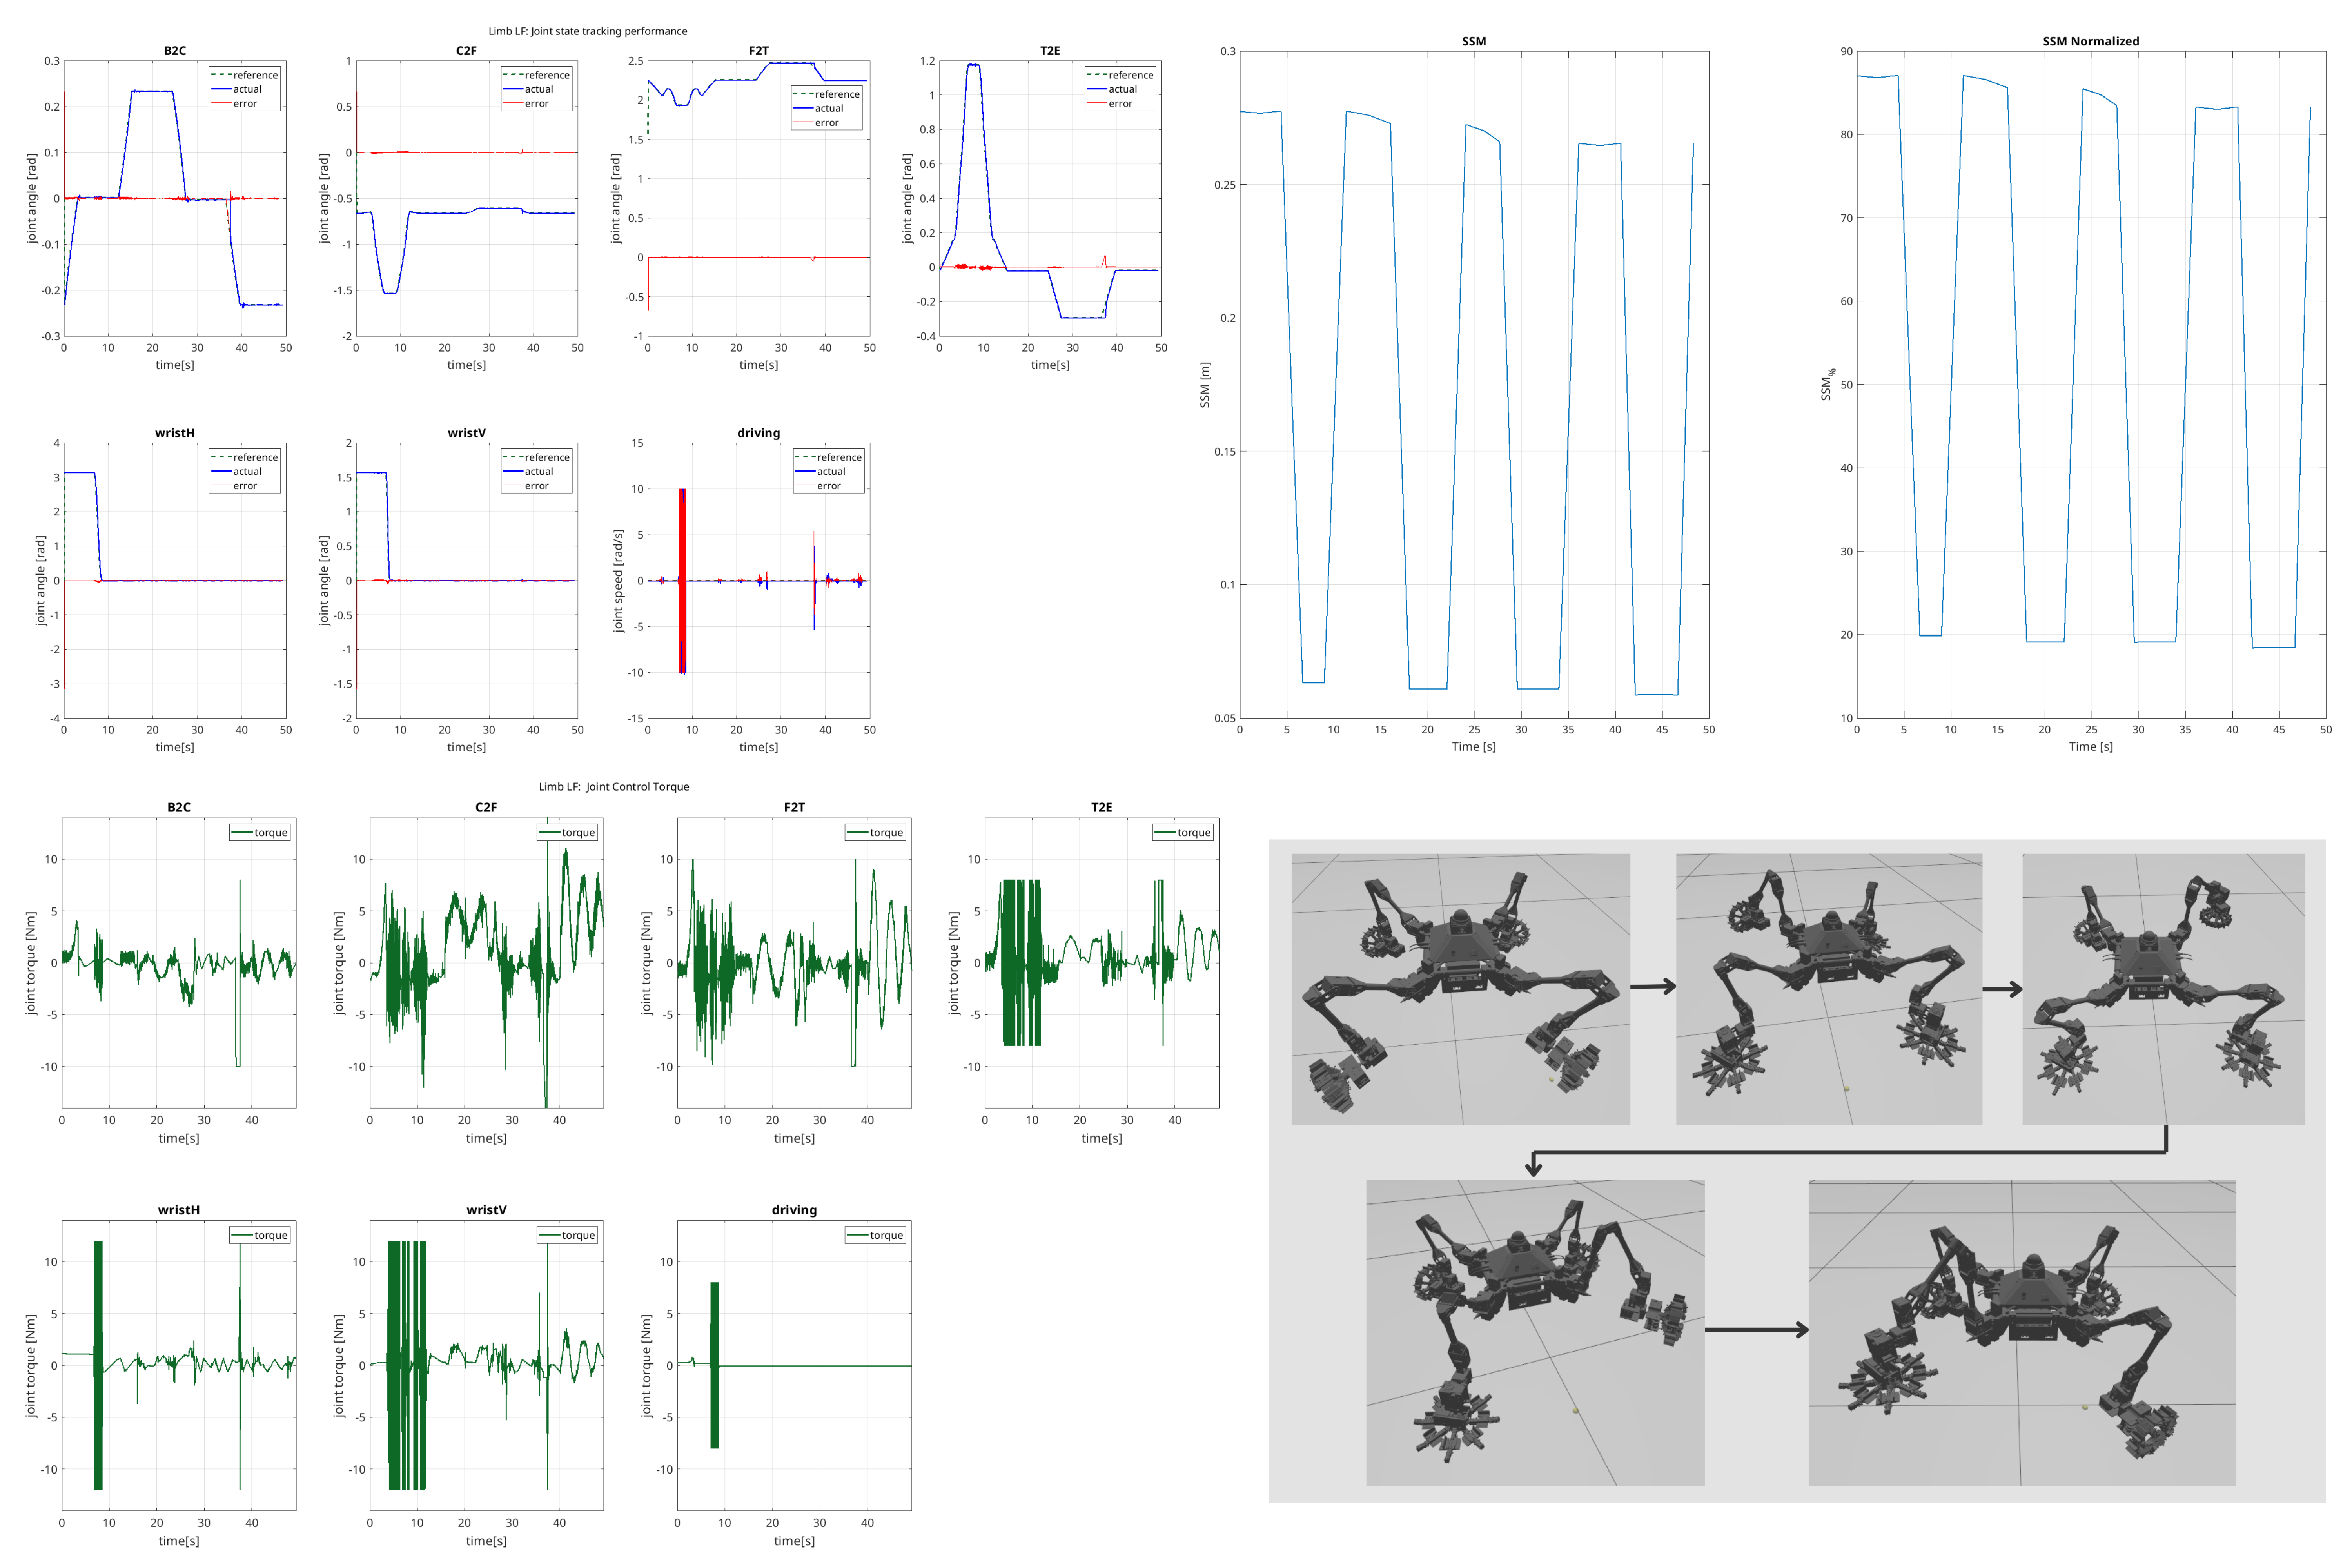
\includegraphics[width=0.5\textwidth]{Images/W2G.png}} 
    \caption{Experiment and Simulation Results. Locomotion mode transition is executed maintaining the $SSM_\%$ above the 16\%, with average joint tracking error below $0.05 rad$, and major ATBVME axis parallel to the desired base motion.}
    \label{fig:results}
\end{figure*}

\subsection{Additional Simulations}
\label{subsec:sim1}
In this new environment, the problem of feasible motors' torque has been considered, and complex motion sequences, not possible with the real hardware (as discussed in the next), have been executed.

\begin{itemize}
    \setlength\itemsep{-0.7pt} 
    \item \textbf{IJCs implementation}: The new low-level control infrastructure implemented from scratch is tested.
    \item \textbf{Wheeled Locomotion}: The ability to perform driving forward locomotion is addressed and analyzed, both on three or four support wheels.
    \item \textbf{Locomotion transition}: The transformation of all GRIEEL modules from G2W and vice versa is further investigated.
\end{itemize}
%-----------------------------------------------------------------------------
% RESULTS
%-----------------------------------------------------------------------------
\section{Results and Discussion}
\label{sec:results}
The results of a G2W experiment are shown in Fig.\ref{fig:experimentG2W}, while a W2G in Gazebo Harmonic is reported in Fig.\ref{fig:simulationW2G}. Additionally, in simulation also stable driving locomotion on four and three wheels has been achieved, showing additional effort in the three-wheeled locomotion to maintain stability.
The manipulability during the whole transition sequence is kept with an almost isotropic shape, meaning that the robot is ready to move in any direction. The stability margin is always kept above 15\% for all motions. Finally, also the joint controller tracking performance is satisfactory, with a negligible steady-state error and settling time below 1 second.

The limitations of the real hardware however have been evident during experiments, and a counterweight solution has to be integrated into the setup. Without external base support, limb motor failure occurs. Moreover, results from the simulation show joint torques 5 times higher than the rated torque of the currently employed motors. 



%-----------------------------------------------------------------------------
% CONCLUSION
%-----------------------------------------------------------------------------
\section{Conclusions}
\label{sec:conclusion}

The defined objectives have been completed, and this research contributes to the future autonomy of LIMBERO-GRIEEL in exploring unstructured environments with smooth locomotion transitions. Simple G2W transofrmation has been proven in the real system, and multitasking in simulation. Moreover, a generic theory on multilimbed robot manipulability analysis has been derived, and extensions will be considered. 
For example, intersecting stable regions defined by the GIA polyhedron\cite{GIA_polyedron} with the ATBVME is an interesting future development. Furthermore,  integrating task consistent planning \cite{TaskCompatibilityPosture} and dynamic manipulability is another possible future work. Additionally, the robot actuator limitation and missing feedback information are evident signs of required hardware improvements, already under development at the SRL. 

\vspace{0.5cm}
\begin{tcolorbox}[
      colback=bluepoli!20,
      colframe=bluepoli!40, 
      title=Additional Resources,
      sharp corners=south,
      fonttitle=\bfseries,
      coltitle=bluepoli!90!black,
    ]
    As supplementary resources, the hardware experiments and simulations have been documented in a set of videos on \href{https://youtube.com/playlist?list=PLFgoOtxCJKTPv_dibdvSUT_YPGDJBc_5C&si=bgCxZ_qWpax2N8Xt}{YouTube}.
    Furthermore, the MATLAB code used for limbed robot kinematic, dexterity analysis, and algorithm evaluation is on \href{https://github.com/AlePuglisi/limbed-robot-control}{GitHub}.
\end{tcolorbox}
\vspace{0.5cm}

%-----------------------------------------------------------------------------
% HOW TO CITE BIBLIOGRAPHY
%-----------------------------------------------------------------------------
\section*{Bibliography}
\label{sec:bibliography}

%---------------------------------------------------------------------------
%  BIBLIOGRAPHY
%---------------------------------------------------------------------------
% Remember to insert here only the essential bibliography of your work
\bibliography{executive_summary.bib} % automatically inserted and ordered with this command 

\end{document}



